% ---------------------------------------------------------------------
%
% TRD Software Writeup
%
% ---------------------------------------------------------------------
%
\documentclass{alicetdr}
%\documentclass[draft]{alicetdr}
%
% For figures
\usepackage{graphicx}
%
% Helvetica
\usepackage{helvet}
\renewcommand{\rmdefault}{phv}
\renewcommand{\sfdefault}{phv}
%
\let\Otemize =\itemize
\let\Onumerate =\enumerate
\let\Oescription =\description
% Zero the vertical spacing parameters
\def\Nospacing{\itemsep=0pt\topsep=0pt\partopsep=0pt\parskip=0pt\parsep=0pt}
\def\Topspac{\vspace{-0.5\baselineskip}}
\def\Botspac{\vspace{-0.2\baselineskip}}
% Redefine the environments in terms of the original values
\newenvironment{Itemize}{\Topspac\Otemize\Nospacing}{\endlist\Botspac}
\newenvironment{Enumerate}{\Topspac\Onumerate\Nospacing}{\endlist\Botspac}
\newenvironment{Description}{\Topspac\Oescription\Nospacing}{\endlist\Botspac}
%
%
% ---------------------------------------------------------------
% define new commands/symbols
% ---------------------------------------------------------------
%
% General stuff
%
\hyphenation{ALICE}
\hyphenation{ATLAS}
\hyphenation{ALSIM}
\hyphenation{SPSLC}
\hyphenation{between}
\hyphenation{basis}
\hyphenation{robust}
\hyphenation{cables}
\hyphenation{below}
\hyphenation{because}
\hyphenation{every rectan-gular}
\newcommand{\Lumi}{\ensuremath{\cal{L}}}
%
\newcommand{\clearemptydoublepage}{\newpage{\pagestyle{empty}\cleardoublepage}}
\newcommand{\HRule}{\rule{0.4\linewidth}{0.3mm}}
\newcommand{\cinst}[2]{$^{\protect\mathrm{#1)}}$~#2\par}
\newcommand{\crefi}[1]{$^{\protect\mathrm{#1)}}$}
\newcommand{\crefii}[2]{$^{\protect\mathrm{#1,#2)}}$}
\newcommand{\Rule}{\rule[-.7ex]{0ex}{2.9ex}}
\newcommand{\rbox}[1]{\raisebox{1.5ex}[-1.5ex]{#1}}
%
% symbols...
%
\newcommand{\mrm}{\mathrm}
\newcommand{\pt}{\ensuremath{p_{\mathrm{t}}} }
\newcommand{\et}{\ensuremath{E_{\mathrm{T}}}}
%\newcommand {\pT} {\mbox{$p_{\rm t}$}}
\newcommand{\mt}{\ensuremath{m_{\mathrm{t}}}}
\newcommand{\minv}{\mbox{$m_{\ee}$}}
\newcommand{\ee}{\mbox{e$^+$e$^-$}}
\newcommand {\rap} {\mbox{$\left | y \right | $}}
%\newcommand{\sigee}{\raisebox{0.2ex}{$\sigma_E$}/\raisebox{-0.4ex}{\kern0.1em$E$}}
\newcommand{\sigee}{$\sigma_E$/$E$}
\newcommand{\dd}{\mrm{d}}
% ... &
\newcommand{\eg}{{e.g.~\@\xspace}}
\newcommand{\ie}{i.e.\@\xspace}
\newcommand{\elm}{e.m.\@\xspace}

%\def\mt{\relax \ifmmode m_{\mathrm{t}} \else $m_{\mathrm{t}}$\@\xspace\fi}
%\def\pt{\relax \ifmmode p_{\mathrm{t}} \else \mbox{$p_{\mathrm{t}}$}\xspace\fi}
%
% units of measure
%
\newcommand {\lum} {\, \mbox{${\rm cm}^{-2} {\rm s}^{-1}$}}
\newcommand {\barn} {\, \mbox{${\rm barn}$}}
\newcommand {\m} {\, \mbox{${\rm m}$}}
\newcommand {\bstar} {\, \mbox{$\beta^{*}$}}
\newcommand {\hour} {\, \mbox{${\rm h}$}}
\newcommand{\dg}{\mbox{$^\circ$}}
%\newcommand {\grad} {\mbox{$^{\circ}$}}
\newcommand {\mass} {\mbox{\rm GeV$\kern-0.15em /\kern-0.12em c^2$}}
\newcommand {\tev} {\mbox{${\rm TeV}$}}
\newcommand {\gev} {\mbox{${\rm GeV}$}}
\newcommand {\mev} {\mbox{${\rm MeV}$}}
\newcommand {\kev} {\mbox{${\rm keV}$}}
\newcommand {\mom} {\mbox{\rm GeV$\kern-0.15em /\kern-0.12em c$}}
\newcommand {\mum} {\mbox{$\mu {\rm m}$}}
\newcommand {\gmom} {\mbox{\rm GeV$\kern-0.15em /\kern-0.12em c$}}
\newcommand {\mmass} {\mbox{\rm MeV$\kern-0.15em /\kern-0.12em c^2$}}
\newcommand {\mmom} {\mbox{\rm MeV$\kern-0.15em /\kern-0.12em c$}}
\newcommand {\nb} {\mbox{\rm nb}}
\newcommand {\musec} {\mbox{$\mu {\rm s}$}}
\newcommand {\cm} {\mbox{${\rm cm}$}}
\newcommand {\mm} {\mbox{${\rm mm}$}}
\newcommand {\cmq} {\mbox{${\rm cm}^{2}$}}
\newcommand {\dens} {\mbox{${\rm g}/{\rm cm}^{3}$}}
%
% Particles
%
\newcommand{\pizero}{\mbox{$\mathrm {\pi^0}$}}
\newcommand{\K}{\mbox{$\mathrm {K}$}}
\newcommand{\Kzs}{\mbox{$\mathrm {K^0_S}$}}
\newcommand{\KzS}{\mbox{$\mathrm {K^0_S}$}}
\newcommand{\KzL}{\mbox{$\mathrm {K^0_L}$}}
\newcommand{\Jpsi} {\mbox{J\kern-0.05em /\kern-0.05em$\psi$}\xspace}
\newcommand{\psip} {\mbox{$\psi^\prime$}\xspace}
\newcommand{\Ups} {\mbox{$\Upsilon$}\xspace}
\newcommand{\Upsp} {\mbox{$\Upsilon^\prime$}\xspace}
\newcommand{\Upspp} {\mbox{$\Upsilon^{\prime\prime}$}\xspace}
\newcommand{\qqbar} {\mbox{$q\bar{q}$}\xspace}

%\newcommand{\qqbar}{\mbox{$\mathrm {q\overline{q}}$}}
\newcommand{\ppbar}{\mbox{$\mathrm {p\overline{p}}$}}
\newcommand{\ccbar}{\mbox{$\mathrm {c\overline{c}}$}}
\newcommand{\bbbar}{\mbox{$\mathrm {b\overline{b}}$}}
\newcommand{\sbbbar}{\mbox{$\scriptstyle\mathrm {b\overline{b}}$}}
\newcommand{\ttbar}{\mbox{$\mathrm {t\overline{t}}$}}
\newcommand{\sttbar}{\mbox{$\scriptstyle\mathrm {t\overline{t}}$}}
\newcommand{\BBbar}{\mbox{$\mathrm {B\overline{B}}$}}
\newcommand{\Bzd}{\mbox{$\mathrm {B^0_d}$}}
\newcommand{\Bbzd}{\mbox{$\mathrm {\overline{B}^0_d}$}}
\newcommand{\Bzs}{\mbox{$\mathrm {B^0_s}$}}
\newcommand{\Bbzs}{\mbox{$\mathrm {\overline{B}^0_s}$}}
\newcommand{\gaga}{\mbox{$\mathrm {\gamma\gamma}$}}
%
% Bibliography stuff
%
\def\NIM#1#2#3{Nucl. Instr. Meth. {\bf #1}\ (#2)\ #3}
\def\IEEE#1#2#3{IEEE Trans. Nucl. Sci. {\bf #1}\ (#2)\ #3}
\def\NP#1#2#3{Nucl. Phys. {\bf #1}\ (#2)\ #3}
\def\PL#1#2#3{Phys. Lett. {\bf #1}\ (#2)\ #3}
\def\PR#1#2#3{Phys. Rev. {\bf #1}\ (#2)\ #3}
\def\PRL#1#2#3{Phys. Rev. Lett. {\bf #1}\ (#2)\ #3}
\def\ZP#1#2#3{Z. Phys. {\bf #1}\ (#2)\ #3}
\def\EJP#1#2#3{Eur. J. Phys. {\bf #1}\ (#2)\ #3}
\def\JPG#1#2#3{J. Phys. G: Nucl. Part. Phys. {\bf #1}\ (#2)\ #3}
\def\RMP#1#2#3{Rev. Mod. Phys. {\bf #1}\ (#2)\ #3}
\def\ARNPS#1#2#3{Ann. Rev. Nucl. Part. Sc. {\bf #1}\ (#2)\ #3}
\def\PRP#1#2#3{Phys. Rep. {\bf #1}\ (#2)\ #3}
\def\RPP#1#2#3{Rep. on Progr. in Phys. {\bf #1}\ (#2)\ #3}
%\def\#1#2#3{ {\bf #1}\ (#2)\ #3}

\def\ALI#1#2{ALICE Internal Note {\sc #1--#2}}
\def\ALIC#1#2#3{ALICE Internal Note {\sc #1--#2 (#3)}}
\def\subNIM{submitted to Nucl. Instr. Meth.}
\def\subIEEE{submitted to IEEE Trans. Nucl. Sci.}
\def\subNP{submitted to Nucl. Phys.}
\def\subPL{submitted to Phys. Lett.}
\def\subPR{submitted to Phys. Rev.}
\def\subPRL{submitted to Phys. Rev. Lett.}
\def\subEJP{submitted to Eur. J. Phys.}
%\def\tosubNIM{to be submitted to Nucl. Instrum. Methods}
%\def\tosubNP{to be submitted to Nucl. Phys.}
%\def\tosubPL{to be submitted to Phys. Lett.}
%\def\tosubPR{to be submitted to Phys. Rev.}
%\def\tosubPRL{to be submitted to Phys. Rev. Lett.}
%\def\tosubZP{to be submitted to Z. Phys.}
%
% Gases
%
\def\xea{\mbox{Xe,CH$_4$ (10\%)}}
\def\xeb{\mbox{Xe,CO$_2$ (10\%)}}
\def\xec{\mbox{Xe,CO$_2$ (15\%)}}
\def\xed{\mbox{Xe,CO$_2$ (20\%)}}
%
% other things...
%
\def\tvi{\vrule height 12pt depth 5pt width 0pt}
\def\vphant{\vphantom{{{1\over{2}}\over{{1\over{2}}}}}}
\def\dis{\displaystyle}

\newlength{\digitwidth} \settowidth{\digitwidth}{\rm 0}
\newlength{\ql} \newlength{\qll} \newlength{\qlll}  \newlength{\qllll}
\newlength{\qlp} \newlength{\qllp} \newlength{\qlllp} \newlength{\qllllp}
\settowidth{\ql}{0} \settowidth{\qll}{00} \settowidth{\qlll}{000}  \settowidth{\qllll}{0000}
\settowidth{\qlp}{.0} \settowidth{\qllp}{.00} \settowidth{\qlllp}{.000} \settowidth{\qllllp}{.0000}
\newlength{\qlup} \newlength{\qlupp}
\settowidth{\qlup}{$^{\prime}$} \settowidth{\qlupp}{$^{\prime\prime}$}
%
% ---------------------------------------------------------
% - End of Definitions
% ---------------------------------------------------------









%
\begin{document}
%
\pagenumbering{roman}
%
%%%%%%%%%%%%%%%%%%%%%%%%%%%%%%%%%%%%%%%%%%%%%%%%%%%%%%%%%%%%%%%%%%%%%
%
% Title page
%
\font\HUGEA=phvr at 36mm  % declare very big font
\font\HUGEB=phvr at 14mm  % declare very big font
%
\begin{titlepage}
%
\vspace{10.0cm}
%
\begin{center}
{\HUGEA T\hspace{5.mm}R\hspace{5.mm}D} \\
%
\vspace{3.5cm}
{\HUGEB Offline Software Writeup} \\
%
\vspace{2.0cm}
{\Large Version 1.0, \today}\\
%
\vfill
%
\vspace{5.5cm}
%
\end{center}
%
\end{titlepage}
%
%%%%%%%%%%%%%%%%%%%%%%%%%%%%%%%%%%%%%%%%%%%%%%%%%%%%%%%%%%%%%%%%%%%%%
%
% Empty page to adjust page numbering
%
\onecolumn
\thispagestyle{empty}
\mbox{  }
%
\setcounter{page}{0}
\onecolumn
%
%%%%%%%%%%%%%%%%%%%%%%%%%%%%%%%%%%%%%%%%%%%%%%%%%%%%%%%%%%%%%%%%%%%%%
%
\pagenumbering{arabic}
%
%%%%%%%%%%%%%%%%%%%%%%%%%%%%%%%%%%%%%%%%%%%%%%%%%%%%%%%%%%%%%%%%%%%%%
%
% List of content
%
%%%%%%%%%%%%%%%%%%%%%%%%%%%%%%%%%%%%%%%%%%%%%%%%%%%%%%%%%%%%%%%%%%%%%
%
\thispagestyle{empty}
\tableofcontents
%
%%%%%%%%%%%%%%%%%%%%%%%%%%%%%%%%%%%%%%%%%%%%%%%%%%%%%%%%%%%%%%%%%%%%%
%
% Text
%
%%%%%%%%%%%%%%%%%%%%%%%%%%%%%%%%%%%%%%%%%%%%%%%%%%%%%%%%%%%%%%%%%%%%%
%
%%%%%%%%%%%%%%%%%%%%%%%%%%%%%%%%%%%%%%%%%%%%%%%%%%%%%%%%%%%%%%%%%%%%%
\newpage
\setcounter{chapter}{0}
\setcounter{section}{0}    
\Chapter{Introduction}
\thispagestyle{empty}
%
This document is supposed to provide a description of the offline
software components that are specific to the TRD.  It is an attempt
to collect useful informations on the design and usage of the TRD
software, in order to facilitate newcomers the introduction to the
code.  The most important classes and procedures are described and
several examples and use cases are given.
However, this writeup is not meant to be a basic AliRoot introduction.  
For this purpose the reader is referred to the general AliRoot users 
guide \cite{ALIROOT}. 
%
%%%%%%%%%%%%%%%%%%%%%%%%%%%%%%%%%%%%%%%%%%%%%%%%%%%%%%%%%%%%%%%%%%%%%
\newpage
\setcounter{chapter}{1}
\setcounter{section}{0}    
\Chapter{Simulation}
\thispagestyle{empty}
%
\section{Geometry}
\label{GEO:intro}
%
{\it Author: C.~Blume (blume@ikf.uni-frankfurt.de)}
\smallskip
\\
%
The TRD geometry, as implemented in {\tt AliTRDgeometry}, consists of 
several components: The readout chambers (ROC), the services, and the 
supermodule frame.  All these parts are placed inside the TRD mother 
volumes, which in turn are part of the space frame geometry 
({\tt AliFRAMEv2}).  Therefore, the space frame geometry has to be 
present to build the TRD geometry.  For each of the 18 supermodules 
one single mothervolume is provided (BTRDxx).  This allows to configure 
the TRD geometry in {\tt Config.C} such that it only contains a subset 
of supermodules in the total ALICE geometry via 
{\tt AliTRDgeometry::SetSMstatus()}.  An incomplete detector setup, as
it exists for first data taking, can thus be modelled.  The class
{\tt AliTRDgeometry} also serves as the central place to collect all
geometry relevant numbers and the definitions of various numbering
schemes of detector components (e.g. sector numbers).  However, all 
geometric parameters that refer to the pad planes are compiled in
{\tt AliTRDpadPlane}.
%
\subsection{Readout Chambers}
\label{GEO:rocs}
%
\begin{figure}[htb]
\begin{center}
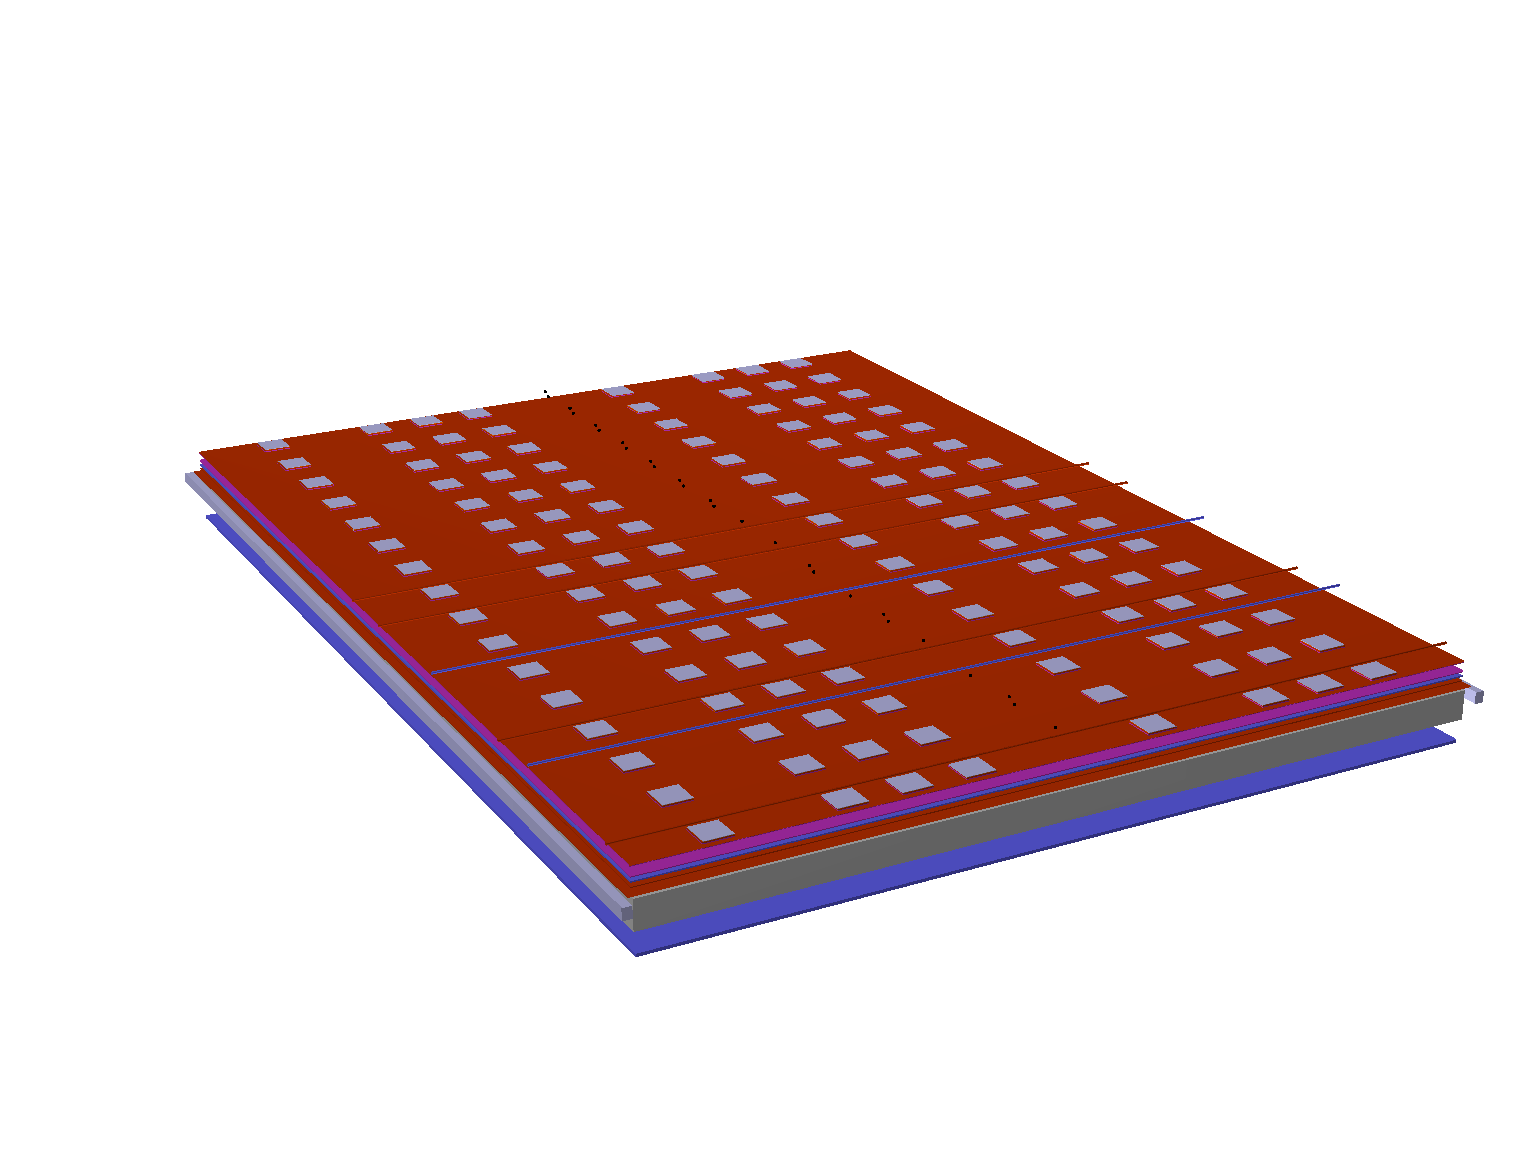
\includegraphics[width=0.85\textwidth]{plots/geo_roc.eps}
\end{center}
\caption{
A TRD read out chamber as implemented in the AliRoot geometry.  The
various material layers are visible.  Also, the MCMs on top of the
chamber, as well as the cooling pipes are shown.
}
\label{FIG_GEO:roc_geom}
\end{figure}
%
All ROCs are modelled in the same way, only their dimensions vary.  
They consist of an aluminum frame, which contains the material for 
the radiator and the gas of the drift region, a Wacosit frame (whose 
material is represented by carbon), that surrounds the amplification 
region, and the support structure, consisting of its aluminum frame, 
material for the read out pads, back panel, and readout boards).  The 
material inside the active parts of the chambers (radiator, gas, wire 
planes, pad planes, glue, read out boards, etc.) is introduced by 
uniform layers of the corresponding material, whose thicknesses were 
chosen such to result in the correct radiation length.  On top of the
individual ROCs the multi chip modules (MCM) as well as the cooling 
pipes and cables are placed.  One obvious simplification, already visible
in Fig.~\ref{FIG_GEO:roc_geom}, is that in the AliRoot geometry the pipes
run straight across the chambers instead of following the meandering path 
as in reality.
%
\subsection{Supermodules}
\label{GEO:smframes}
%
\begin{figure}[htb]
\begin{center}
\begin{minipage}[b]{0.49\textwidth}
\begin{center}

\includegraphics[width=0.65\textwidth,angle=270]{plots/geo_smframe.eps}
\end{center}
\end{minipage}
\begin{minipage}[b]{0.49\textwidth}
\begin{center}
\includegraphics[width=0.70\textwidth,angle=270]{plots/geo_sm.eps}
\end{center}
\end{minipage}
\end{center}
\caption{
A TRD supermodule, as implemented in the AliRoot geometry.  The left
panel shows only the support structures of the aluminum frame, together
with some service elements.  The right panel shows a complete 
supermodule including some surrounding parts of the space frame.
}
\label{FIG_GEO:sm_geom}
\end{figure}
%
The supermodule frames consist of the aluminum sheets on the sides, top,
and bottom of a supermodule together with the traversing support structures.
The left panel of Fig.~\ref{FIG_GEO:sm_geom} shows the structures that are
implemented in the TRD geometry.  Also, parts of the services like the LV
power bus bars and cooling arteries can be seen.  Additional electronics 
equipment (e.g. ``Sch\"utten-Box``) is represented by aluminum boxes that 
contain corresponding copper layers to mimic the present material.  The 
services also include e.g. gas distribution boxes, cooling pipes, power and
readout cables, and power connection panels.  Part of the services extend
into the baby and the back frame.  Therefore, additional mother volumes
have been introduced in order to accommodate this material.  All supermodules 
have inserts of carbon fiber sheets in the bottom part of the aluminum 
casing, for the ones in front of the PHOS detector (sectors 11--15) also 
the top part includes carbon fiber inserts.  The supermodules in the sectors 
13--15 do not contain any ROCs in the middle stack in order to provide the 
holes for the PHOS detector.  Instead, gas tubes of stainless steel have
been built in.
%
Generally, the TRD volumina start with the letter  ``{\bf U}''.  The geometry
is defined by the function {\tt AliTRDgeometry::CreateGeometry()}, which
generates the TRD mother volumes ({\bf UTI1}, {\bf UTI2}, {\bf UTI3}) and the 
volumes that constitute a single ROC.  This function in turn also calls 
{\tt AliTRDgeometry::CreateFrame()} to create the TRD support frame, 
{\tt AliTRDgeometry::CreateServices()} to create the services, and 
{\tt AliTRDgeometry::GroupChambers()} which assembles the alignable
volumes for a single ROC ({\bf UTxx}, where {\bf xx} is the detector
number {\bf DET-SEC}, defined inside a single super module, see below). The
materials, together with their tracking parameters, that are assigned to
the volumina, are defined in {\tt AliTRD::CreateMaterials()}.
In the following table the most important TRD volumina are described
({\bf xx} = {\bf DET-SEC} number):
%
\begin{center}
\begin{tabular}{l|l}
Name       & Description                                                                \\ \hline
{\bf UTR1} & TRD mothervolume for default supermodules                                  \\
{\bf UTR2} & TRD mothervolume for supermodules in front of PHOS                         \\
{\bf UTR3} & As {\bf UTR2}, but w/o middle stack                                        \\ \hline
{\bf UTxx} & Top volume of a single ROC                                                 \\ 
           & Defines the alignable volume for a single ROC                              \\ \hline
{\bf UAxx} & Lower part of the ROCs, including drift volume and radiator                \\
{\bf UDxx} & Amplification region                                                       \\
{\bf UFxx} & Back panel, including pad planes and PCB boards of readout electronics     \\
{\bf UUxx} & Contains services on chambers (cooling, cables, DCS boards) and MCM chips  \\
\end{tabular}
\end{center}
%
\subsection{Material Budget and Weight}
%
\begin{figure}[htb]
\begin{center}
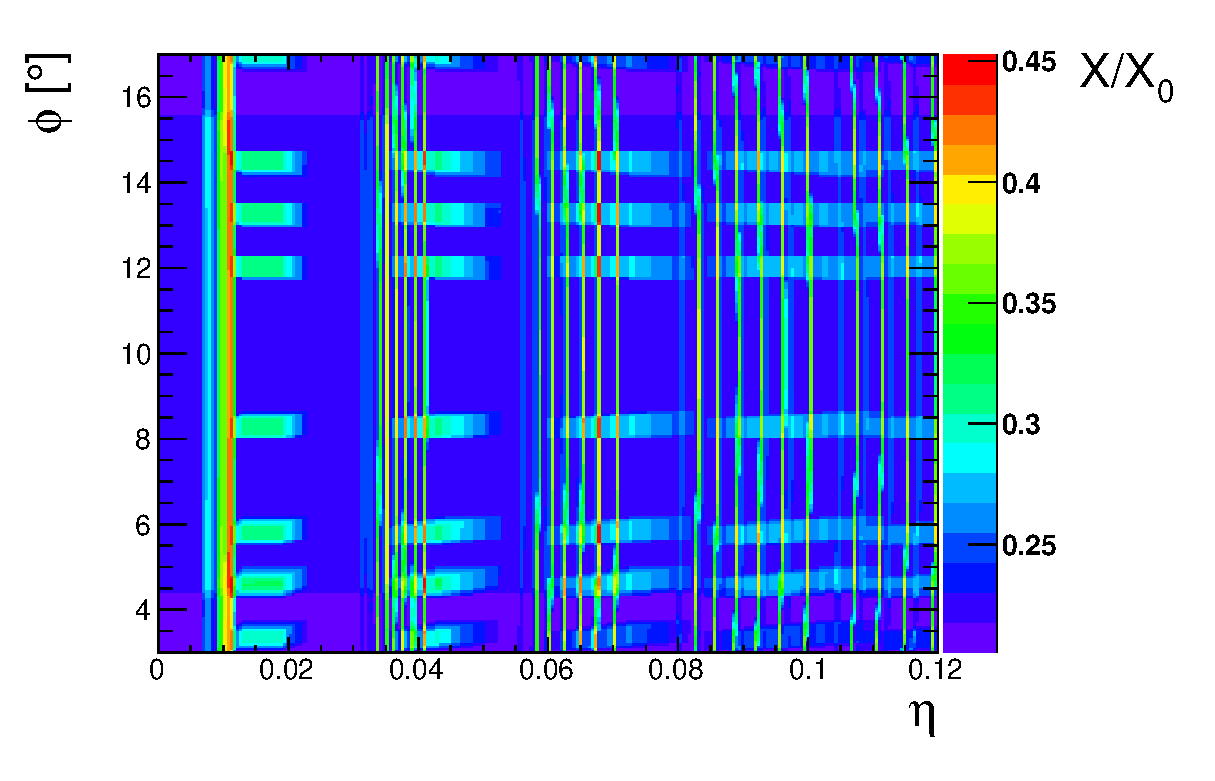
\includegraphics[width=0.75\textwidth]{plots/geo_material_budget.eps}
\end{center}
\caption{
The radiation length map in units of $X/X_{0}$ in part of the active 
detector area of super module 0 as a function of the pseudorapidity 
$\eta$ and the azimuth angle $\phi$, calculated from the geometry in 
AliRoot.  Visible are the positions of the MCMs and the cooling pipes 
as hot spots.
}
\label{FIG_GEO:mat_budget}
\end{figure}
%
The volumina defining a ROC contain several layers that represent the 
different materials present inside a chamber and which therefore define 
the material budget inside the sensitive areas:
\begin{center}
\begin{tabular}{l|l|l|l|c|c|c}
Name         & Mother & Material    & Description                  & Thickness & Density      & $X/X_{0}$ \\ 
             &        &             &                              & [cm]      & [g/cm$^{3}$] & [\%]      \\ \hline
{\bf URMYxx} & UAxx   & Mylar       & Mylar layer on radiator (x2) & 0.0015    & 1.39         & 0.005     \\
{\bf URCBxx} & UAxx   & Carbon      & Carbon fiber mats (x2)       & 0.0055    & 1.75         & 0.023     \\
{\bf URGLxx} & UAxx   & Araldite    & Glue on the fiber mats (x2)  & 0.0065    & 1.12         & 0.018     \\
{\bf URRHxx} & UAxx   & Rohacell    & Sandwich structure (x2)      & 0.8       & 0.075        & 0.149     \\
{\bf URFBxx} & UAxx   & PP          & Fiber mats inside radiator   & 3.186     & 0.068        & 0.490     \\ \hline
{\bf UJxx}   & UAxx   & Xe/CO$_{2}$ & The drift region             & 3.0       & 0.00495      & 0.167     \\ 
{\bf UKxx}   & UDxx   & Xe/CO$_{2}$ & The amplification region     & 0.7       & 0.00495      & 0.039     \\ 
{\bf UWxx}   & UKxx   & Copper      & Wire planes (x2)             & 0.00011   & 8.96         & 0.008     \\ \hline
{\bf UPPDxx} & UFxx   & Copper      & Copper of pad plane          & 0.0025    & 8.96         & 0.174     \\
{\bf UPPPxx} & UFxx   & G10         & PCB of pad plane             & 0.0356    & 2.0          & 0.239     \\
{\bf UPGLxx} & UFxx   & Araldite    & Glue on pad plane            & 0.0923    & 1.12         & 0.249     \\
             &        & Araldite    & + additional glue (leaks)    & 0.0505    & 1.12         & 0.107     \\
{\bf UPCBxx} & UFxx   & Carbon      & Carbon fiber mats (x2)       & 0.019     & 1.75         & 0.078     \\
{\bf UPHCxx} & UFxx   & Aramide     & Honeycomb structure          & 2.0299    & 0.032        & 0.169     \\
{\bf UPPCxx} & UFxx   & G10         & PCB of readout boards        & 0.0486    & 2.0          & 0.326     \\
{\bf UPRDxx} & UFxx   & Copper      & Copper of readout boards     & 0.0057    & 8.96         & 0.404     \\
{\bf UPELxx} & UFxx   & Copper      & Electronics and cables       & 0.0029    & 8.96         & 0.202     \\
\end{tabular}
\end{center}
This material budget has been adjusted to match the estimate given 
in~\cite{CLEMENS}, with the exception of the glue layer in the back panel
({\bf UPGLxx}), which has been made thicker to include all the additional
glue that has been applied to fix the gas leaks.  Figure~\ref{FIG_GEO:mat_budget}
shows the resulting radiation length map in the active detector area for
super module 0, which has only carbon fiber inserts at the bottom and is
thus one of the super modules with the largest material budget.  It is
clearly visible that the MCMs and the cooling pipes introduce hot spots
in $X/X_{0}$.  However, after averaging over the shown area, the mean
value is found to be $\langle X/X_{0}\rangle =$~24.7~\%.  For a supermodule
with carbon fiber inserts at the top and the bottom one finds
$\langle X/X_{0}\rangle =$~23.8~\% and in the regions of the PHOS holes (i.e.
in the middle stack of supermodules 13--15) it is only 
$\langle X/X_{0}\rangle =$~1.9~\%.

The total weight of a single TRD super module in the AliRoot geometry, 
including all services, is currently 1595kg, which is ca. 5\% short of its
real weight.  A single ROC of the type L0C1 with electronics and cooling 
pipes weighs 21.82kg.
%
\subsection{Naming Conventions and Numbering Schemes}
%
\begin{figure}[htb]
\begin{minipage}[b]{0.49\textwidth}
\begin{center}
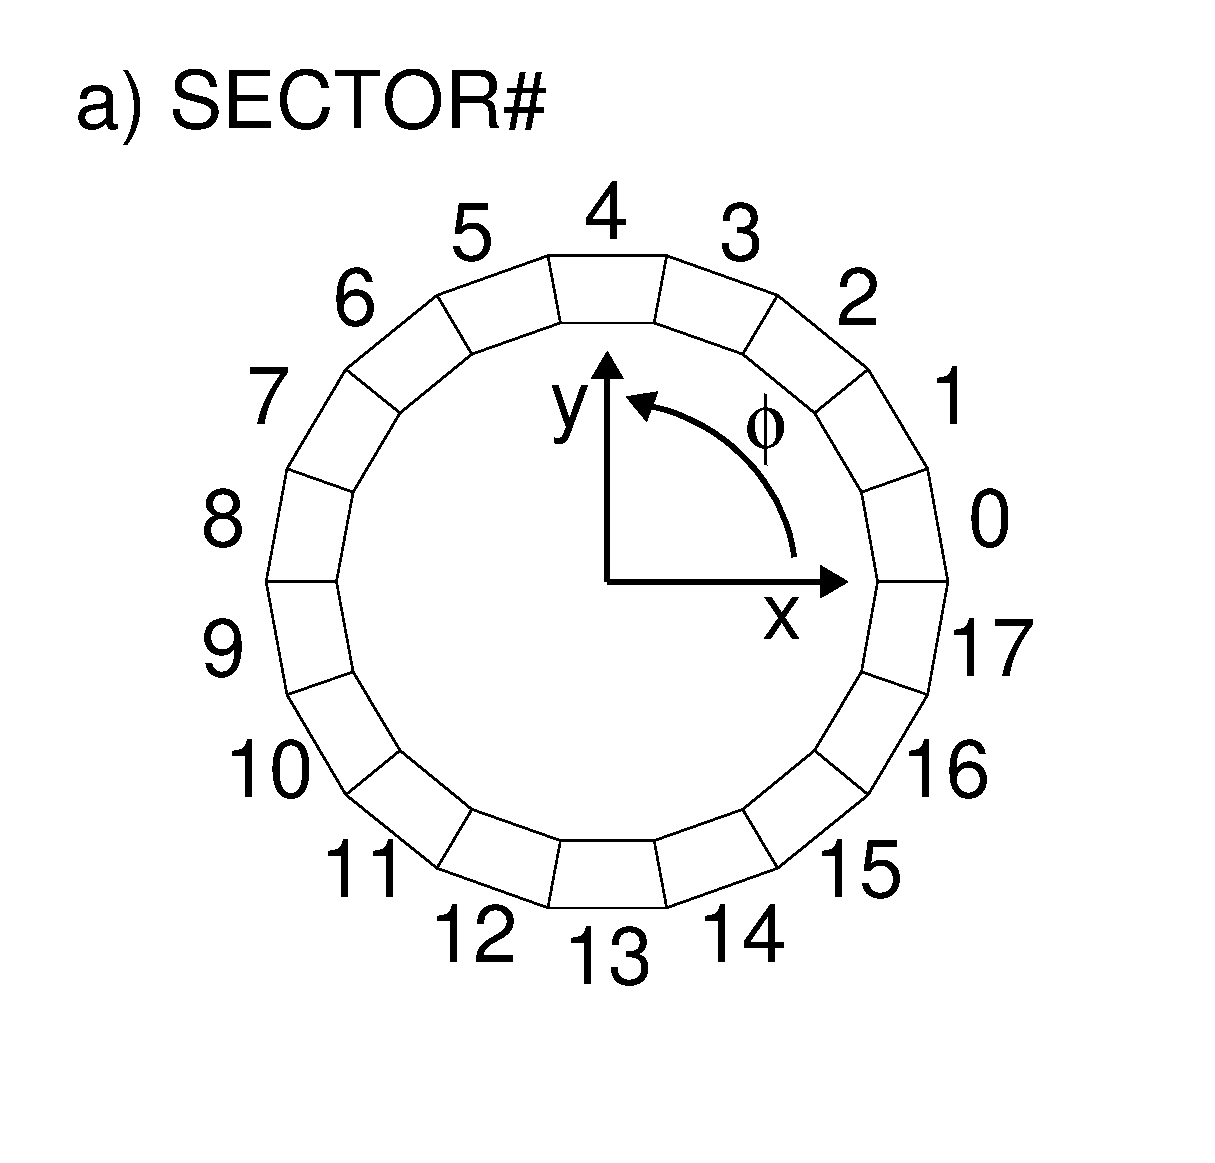
\includegraphics[width=\textwidth]{plots/sector_numbering.eps}
\end{center}
\end{minipage}
\begin{minipage}[b]{0.49\textwidth}
\begin{center}
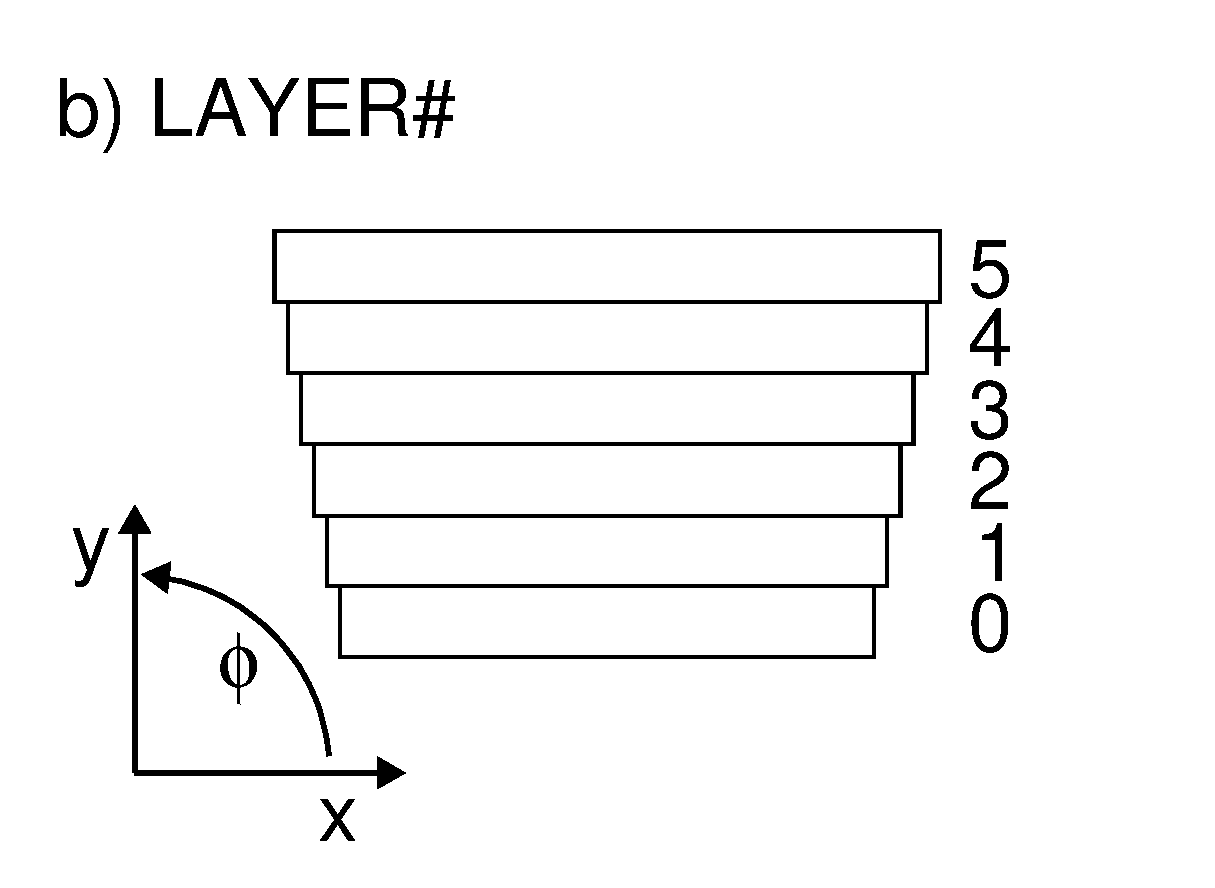
\includegraphics[width=\textwidth]{plots/layer_numbering.eps}
\vspace{1.4cm}
\end{center}
\end{minipage}
\begin{center}
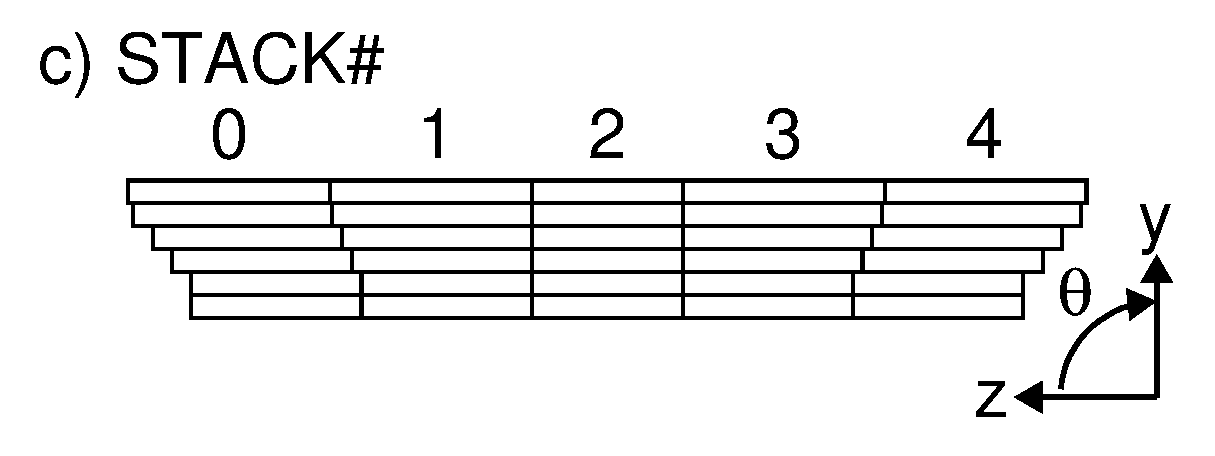
\includegraphics[width=0.60\textwidth]{plots/stack_numbering.eps}
\end{center}
\caption{
Illustration of the TRD numbering scheme for super modules, defined in
the global ALICE coordinate system: a) {\bf SECTOR} number, b) 
{\bf LAYER} number, c) {\bf STACK} number.
}
\label{FIG_GEO:sm_numbering}
\end{figure}
%
The numbering schemes and the orientations of coordinate systems generally 
follow the official ALICE-TRD definition \cite{DAVID}.  Therefore, the
whole geometry is defined in the global ALICE coordinate system.
%
Inside the code we use the following nomenclature (see 
Fig.~\ref{FIG_GEO:sm_numbering}), which should be used consistently
throughout the TRD code:
%
\begin{center}
\begin{tabular}{l|l|l}
Name          & Definition                                   & Range  \\ \hline
{\bf SECTOR}  & TRD sector in azimuth (i.e. one supermodule) & 0--17  \\
{\bf LAYER}   & Layer inside a supermodule                   & 0--5   \\
{\bf STACK}   & Division of a supermodule along z-direction  & 0--4   \\
{\bf DET}     & Single ROC in whole TRD                      & 0--539 \\ 
{\bf DET-SEC} & Single ROC in one super module               & 0--29 
\end{tabular}
\end{center}
%
Due to the holes in front of the PHOS detector, naturally not all {\bf DET} 
numbers correspond to existing ROCs.  A single ROC can thus be uniquely 
addressed by either using the three numbers 
({\bf LAYER}, {\bf STACK}, {\bf SECTOR}) or the single {\bf DET} number.
The correspondence between the two possibilities is defined as:
\begin{center}
\mbox{{\bf DET} = {\bf LAYER} + {\bf STACK}$\times$5 + {\bf SECTOR}$\times$5$\times$4}
\end{center}
Additionally, there is a number that is unique inside a given super module (i.e. 
sector) and therefore has a range of 0~--~29:
\begin{center}
\mbox{{\bf DET-SEC} = {\bf LAYER} + {\bf STACK}$\times$5}
\end{center}
The class {\tt AliTRDgeometry} provides a set of functions that could/should
be used to convert the one into the other:\\
\hspace*{1.5cm}{\tt AliTRDgeometry::GetDetector(layer,stack,sector)} \\
\hspace*{1.5cm}{\tt AliTRDgeometry::GetDetectorSec(layer,stack)}     \\
\hspace*{1.5cm}{\tt AliTRDgeometry::GetLayer(det)}                   \\
\hspace*{1.5cm}{\tt AliTRDgeometry::GetStack(det)}                   \\
\hspace*{1.5cm}{\tt AliTRDgeometry::GetSector(det)}                  \\
%
\subsection{Pad Planes}
%
All geometric parameters relevant to the pad planes are handled via the
class {\tt AliTRDpadPlane}.  This comprises the dimensions of the pad planes
and the pad themselves, the number of padrows, padcolumns, and their tilting angle.  
The initialization of the needed {\tt AliTRDpadPlane} objects is done in 
{\tt AliTRDgeometry::CreatePadPlaneArray()}.  The number of padrows can be 12 
(C0-type) or 16 (C1-type), the number of padcolumns is 144 in any case.  Again,
the numbering convention follows the definition given in \cite{DAVID}.  Thus,
the padrow numbers in a given pad plane increase from 0 to 11(15) with decreasing
$z$-position, while the padcolumn numbers increase from 0 to 144 with increasing 
$\phi$ angle (i.e. counter clockwise).  The tilting angle of the pads is 2~degrees,
with alternating signs at different layers, beginning with +2~degrees for layer~0.
The class {\tt AliTRDpadPlane} provides a variety of functions that allow to assign 
a pad number (row/column) to signals generated at a given hit position and which
are used during the digitization process.
%
\section{Hit Generation}
%
{\it Author: C.~Blume (blume@ikf.uni-frankfurt.de)}
\smallskip
\\
%
In the case of the TRD a single hit corresponds to a cluster of electrons 
resulting from the ionization of the detector gas.  This ionization can be due
to the normal energy loss process of a charged particle or due to the 
absorption of a transition radiation (TR) photon.  A single TRD hit, as
defined in {\tt AliTRDhit} therefore contains the following data members:
%
\begin{center}
\begin{tabular}{ll}
{\tt fTrack}    & Index of MC particle in kine tree                                        \\
{\tt fX}        & X-position of the hit in global coordinates                              \\
{\tt fY}        & Y-position of the hit in global coordinates                              \\
{\tt fZ}        & Z-position of the hit in global coordinates                              \\
{\tt fDetector} & Number of the ROC ({\bf DET} number)                                     \\
{\tt fQ}        & Number of electrons created in the ionization step. Negative for TR hits \\
{\tt fTime}     & Absolute time of the hit in $\mu$s. Needed for pile-up events            \\
\end{tabular}
\end{center}
%
On top of this, it is also stored in the {\tt TObject} bit field status word  
whether a hit is inside the drift or the amplification region 
(see {\tt AliTRDhit::FromDrift()} and {\tt AliTRDhit::FromAmplification()}).
The creation of hits is steered by {\tt AliTRDv1::StepManager()}.
%
\subsection{Energy loss}
%
A charged particle, traversing the gas volume of the TRD chambers, will release
charge proportional to its specific energy loss.  In the TRD code this process
is implemented in \\{\tt AliTRDv1::StepManager()}.  This implementation used a 
fixed step size.  The standard value here is 0.1~cm, but other values can be
set via {\tt AliTRDv1::SetStepSize()}.  The energy deposited in a given step is
then calculated by the chosen MC program (typically Geant3.21), which after
division by the ionization energy gives the number of electrons of the new hit.
The version 2) will also work for an Ar/CO$_{2}$ mixture, which can be selected
by \\{\tt AliTRDSimParam::SetArgon()}. 
%
\subsection{Photons from transition radiation}
%
Additionally to the hits from energy loss, also hits from the absorption of
TR photons are generated.  This is done in {\tt AliTRDv1::CreateTRhit()}, which
in turn is called by the chosen step manager for electrons and positrons
entering the entering the drift volume.  The process consists of two steps:
first the number and energies of the TR photons have to be determined and then
their absorption position inside the gas volume has to be calculated.  The
corresponding procedures, used by {\tt AliTRDv1::CreateTRhit()}, are 
implemented in {\tt AliTRDsimTR()}.  This class contains a parametrization
of TR photons generated by a regular foil stack radiator \cite{TRPHOT}.  This
parametrization has been tuned such that the resulting spectrum matches the
one of the fiber radiator that used in reality.  Since the TR production
depends also on the momentum of the electron, the parameters have been 
adjusted in several momentum bins.  After a TR photon has been generated and put
on the particle stack, it is assumed that it follows a straight trajectory 
whose direction is determined by the momentum vector of the generating electron.  
Since the emission angle for TR photons is very small ($\sim 1/\gamma$) this 
is a valid approximation.  The absorption length, which thus determines the 
TR hit position, is randomly chosen according to the absorption cross sections
in the gas mixture.  These energy dependent cross sections are also included
in {\tt AliTRDsimTR}.
%
\subsection{Track references}
%
The TRD simulation produces track references ({\tt AliTrackReference}) each time 
a charged particle is entering the drift region and exiting the amplification 
region.  These track references thus provide information on the position where 
the MC particle was entering and existing the sensitive region of a ROC, as well
as on its momentum components at this positions.  Also, the index to the MC particle
in the kinematic tree is stored so that the full MC history can be retrieved.
%
\section{Digitization}
%
{\it Author: C.~Blume (blume@ikf.uni-frankfurt.de)}
\smallskip
\\
%
The second step in the simulation chain is the translation of the hit information,
i.e. position and amount of deposited charge, into the final detector response
that can be stored in digits objects ({\tt AliTRDdigits}):
%
\begin{center}
\begin{tabular}{ll}
{\tt fAmp}         & Signal amplitude                      \\
{\tt fId}          & Number of the ROC ({\bf DET} number)  \\
{\tt fIndexInList} & Track index                           \\
{\tt fRow}         & Pad row number                        \\
{\tt fColumn}      & Pad column number                     \\
{\tt fTime}        & Time bin number                       \\
\end{tabular}
\end{center}
%
However, in practice {\tt AliTRDdigits} is not used to store the digits 
information.  Instead the data containers described in \ref{DIGITS:containers}
are used for this purpose.  The digitization process includes as an 
intermediate step between hit and digits the so-called summable digits, or 
sdigits:
\begin{center}
\mbox{{\bf HITS} $\Longrightarrow$ {\bf SDIGITS} $\Longrightarrow$ {\bf DIGITS}}
\end{center}
They sdigits contain the detector signals before discretization and the addition
of noise and are used to merge several events into a single one.
%
\subsection{Digitizer}
%
The class {\tt AliTRDdigitizer} contains all the necessary procedures to convert
hits into sdigits and subsequently sdigits into digits.  The standard sequence to
produce sdigits, as would be initiated by {\tt AliSimulation}, is shown here:
%
\begin{center}
\unitlength1.0cm
\begin{picture}(10,9)
\put(2.5,8.0){\framebox(5.0,0.8){{\tt MakeDigits()}}}
\put(2.5,6.4){\framebox(5.0,0.8){{\tt SortHits()}}}
\put(2.5,4.8){\framebox(5.0,0.8){{\tt ConvertHits(det)}}}
\put(2.5,3.2){\framebox(5.0,0.8){{\tt ConvertSignals(det)}}}
\put(2.5,1.6){\framebox(5.0,0.8){{\tt Signal2SDigits(det)}}}
\put(2.5,0.0){\framebox(5.0,0.8){{\tt TRD.SDigits.root}}}
\put(5.0,8.0){\vector(0,-1){0.8}}
\put(5.0,6.4){\vector(0,-1){0.8}}
\put(5.0,4.8){\vector(0,-1){0.8}}
\put(5.0,3.2){\vector(0,-1){0.8}}
\put(5.0,1.6){\vector(0,-1){0.8}}
\put(5.0,1.2){\line(-1,0){4.0}}
\put(1.0,1.2){\line(0,1){4.8}}
\put(1.0,6.0){\vector(1,0){4.0}}
\put(0.2,6.1){{\tt det=0-539}}
\end{picture}
\end{center}
%
The first function {\tt SortHits()} sorts the simulated hits according to
their {\bf DET} number, so that the digitization procedures can be called
for a single ROCs in the following loop.  The function {\tt ConvertHits()}
does the conversion of the hit information into a detector signal.  In this
procedure each electron of a given hit is in principle followed along its
path from the position of the primary ionization towards the anode wire.
The position of this electron can be modified by diffusion in the gas
({\tt AliTRDdigitizer::Diffusion()}), ExB effect ({\tt AliTRDdigitizer::ExB()}),
and absorption ({\tt AliTRDdigitizer::Absorbtion()}, off per default).
The drift time of the electrons is also modified according to their distance
to the corresponding anode wire position ({\tt AliTRDdigitizer::TimeStruct()}),
since the electric field lines are not uniform inside the amplification region.
This results in a non-isochronity of the drift time, which has been
simulated with the GARFIELD program and the tabulated results of this
simulation are used in the digitizing process to adjust the drift times
accordingly. Once the position and the drift time of the electron at the
anode wire plane are know, the signal induced on the pads can be calculated.
This involves three effects: the pad response, which distributes the charge
on several pads ({\tt AliTRDdigitizer::PadResponse()}), the time response due 
to the slow ion drift and the PASA response function, which distributes the
charge onto the following time bins, ({\tt AliTRDdigitizer::TimeResponse()}), 
and the cross talk between neighboring pads {\tt AliTRD\-digitizer::CrossTalk()}).  
At the end of this procedure, the charge seen by each pad in each time bin 
is available.  Also, the indices of maximally three MC particles in the kine
tree contributing to a given pad signal are stored, so that in a later 
analysis it can be tested which particle generated what signal.
As a next step the signals could either directly be converted into {\bf DIGITS},
or, which is the default procedure, they are stored as {\bf SDIGITIS}.
The corresponding functions ({\tt AliTRDdigitizer::Signal2SDigits()} and
{\tt AliTRDdigitizer::Signal2ADC()}) are called from 
{\tt AliTRDdigitizer::ConvertSignals()}, depending on the configuration.
The function {\tt AliTRDdigitizer::Signal2SDigits()} stores the signals as 
{\bf SDIGITS} in data structures of the type {\tt AliTRDarraySignal} (see 
section \ref{DIGITS:containers}).  

If desired, the {\bf SDIGITS} can now be added to the {\bf SDIGITS} from other
simulated events, e.g. in order to embed a specific signal into a background
event ({\tt AliTRDdigitizer::MergeSDigits()}). After this optional step, the 
{\bf SDIGITS} are finally being converted into {\bf DIGITS}. This process is
steered by the function ({\tt AliTRDdigitizer::ConvertSDigits()}). 
%
\begin{center}
\unitlength1.0cm
\begin{picture}(10,9)
\put(2.5,8.0){\framebox(5.0,0.8){{\tt Exec()}}}
\put(2.5,6.4){\framebox(5.0,0.8){{\tt SDigits2Digits()}}}
\put(2.5,4.8){\framebox(5.0,0.8){{\tt MergeSDigits()}}}
\put(2.5,3.2){\framebox(5.0,0.8){{\tt ConvertSDigits()}}}
\put(2.5,1.6){\framebox(5.0,0.8){{\tt Signal2ADC(det)}}}
\put(2.5,0.0){\framebox(5.0,0.8){{\tt TRD.Digits.root}}}
\put(5.0,8.0){\vector(0,-1){0.8}}
\put(5.0,6.4){\vector(0,-1){0.8}}
\put(5.0,4.8){\vector(0,-1){0.8}}
\put(5.0,3.2){\vector(0,-1){0.8}}
\put(5.0,1.6){\vector(0,-1){0.8}}
\put(5.0,1.2){\line(-1,0){4.0}}
\put(1.0,1.2){\line(0,1){1.6}}
\put(1.0,2.8){\vector(1,0){4.0}}
\put(0.2,2.9){{\tt det=0-539}}
\end{picture}
\end{center}
%
The essential step in the final {\bf SDIGITS} $\Longrightarrow$ {\bf DIGITS} 
conversion is performed by the function {\tt AliTRDdigitizer::Signal2ADC()}. 
Here pad signals, that are stored as floats, are finally translated into 
integer ADC values. This conversion involves a number of parameters: the pad 
coupling and time coupling factors, the gain of the PASA and of the 
amplification at the anode wire, and the input range and baseline of the ADCs. 
The coupling factors take into account that only a fraction of the incoming 
signal is sampled in the digitization process. At this point also the relative 
gain factors derived from the calibration procedures for a given dataset will 
be used to distort the simulated data correspondingly. The noise is generated 
according to a Gaussian distribution of a given width and added to the output. 
Finally, the converted signals are discretize into the ADC values of the 
defined resolution. At this stage also the zero suppression mechanism is applied 
to the simulated ADC values ({\tt AliTRDdigitizer::ZS()}), in order to reduce 
the output volume (see section \ref{DIGITS:zs}). These {\bf DIGITS} can then 
serve as input to the raw data simulation (see section \ref{RAWSIM}).
%
\subsection{Simulation parameter}
%
The parameters that are needed to configure the digitization, are either
read from the OCDB (e.g. calibration gain factors) or are taken from the
parameter class {\tt AliTRDSimParam}. This class contains the default values
of these parameters, but it can be configured in order to test different 
scenarios. The following table lists the available parameters:
%
\begin{center}
\begin{tabular}{lll}
Parameter              & Description                                   & Default value \\ \hline
{\tt fGasGain}         & Gas gain at the anode wire                    & 4000          \\
{\tt fNoise}           & Noise of the chamber readout                  & 1250          \\
{\tt fChipGain}        & Gain of the PASA                              & 12.4          \\
{\tt fADCoutRange}     & ADC output range (number of ADC channels)     & 1023 (10bit)  \\
{\tt fADCinRange}      & ADC input range (input charge)                & 2000 (2V)     \\
{\tt fADCbaseline}     & ADC intrinsic baseline in ADC channels        & 0             \\
{\tt fElAttachProb}    & Probability for electron attachment per meter & 0             \\
{\tt fPadCoupling}     & Pad coupling factor                           & 0.46          \\
{\tt fTimeCoupling}    & Time coupling factor                          & 0.4           \\ \hline
{\tt fDiffusionOn}     & Switch for diffusion                          & kTRUE         \\
{\tt fElAttachOn}      & Switch for electron attachment                & kFALSE        \\
{\tt fTRFOn}           & Switch for time response                      & kTRUE         \\
{\tt fCTOn}            & Switch for cross talk                         & kTRUE         \\
{\tt fTimeStructOn}    & Switch for time structure                     & kTRUE         \\
{\tt fPRFOn}           & Switch for pad response                       & kTRUE         \\
{\tt fGasMixture}      & Switch for gas mixture (0: Xe/CO2, 1: Ar/CO2) & 0             \\
\end{tabular}
\end{center}
%
\subsection{Digits manager}
\label{DIGITS:manager}
%
{\it Author: H.~Leon~Vargas (hleon@ikf.uni-frankfurt.de)}
\smallskip
\\
%
The class {\tt AliTRDdigitsManager} handles arrays of data container 
objects in the form of ROOT's {\tt TObjArray}.  Its main functionality 
is that it provides setters and getters for the information of each chamber.
%
\begin{figure}[htb]
\begin{center}

\includegraphics[width=0.85\textwidth]{plots/digitsmanager_containers.eps}
\end{center}
\caption{
Data containers used in the class {\tt AliTRDdigitsManager}.
}
\label{FIG_DIG:manager}
\end{figure}
%
\subsection{Data containers}
\label{DIGITS:containers}
%
During simulation different kinds of information are created and stored 
in various data containers depending on their characteristics. 
These containers were designed with the idea of keeping the code as 
simple as possible and to ease its maintenance. 
The simulated signals or sdigits for a given row, column and time bin 
of each detector, as generated by \\ {\tt AliTRDdigitizer::ConvertHits()}, 
are stored in an object of the class {\tt AliTRDarraySignal}.   This 
class stores the data in an array of floating point values.  In this 
case, the compression method takes as an argument a threshold.  All the 
values equal or below that threshold will be set to zero during
compression. The threshold can take any value greater or equal to zero.
The sdigits data is used during event merging.

In the simulation the information about the particles that generated the
hits (index in kine tree) is stored for each detector in an object
of the class {\tt AliTRDarrayDictionary}. In this case the information 
is stored in an array of integer values, which is initialized to -1.
 
In the digitizer, the signals stored in the sdigits are converted 
afterwards into ADC values and kept in objects of the class 
{\tt AliTRDarrayADC}.  This class saves the ADC values in an array of 
short values. The ADC range uses only the first 9 bits, bits 10 to 12 
are used to set the pad status.  An uncompressed object of the class 
{\tt AliTRDarrayADC} should only contain values that are equal or 
greater than -1, because the compression algorithm of this class uses 
all the other negative values in the range of the short data type. The 
value -1 in the data array is used in the simulation to indicate where 
an ADC value was ``zero suppressed''. This is done in this way so we 
are be able to discriminate between real zeroes and suppressed zeroes. 
For the details of the use of pad status refer to the method 
{\tt AliTRDarrayADC::SetPadStatus()} in the implementation file of this class.
%
\subsection{Zero suppression}
\label{DIGITS:zs}
%
{\it Author: H.~Leon~Vargas (hleon@ikf.uni-frankfurt.de)}
\smallskip
\\
%
The zero suppression algorithm was applied at the end of digitization
in order to decrease the size of the digits file. The code is implemented 
in the class {\tt AliTRDmcmSim}.  This algorithm is based on testing 
three conditions on the ADC values of three neighboring pads as seen 
in Fig.~\ref{FIG_DIG:zs} (for more information see the Data Indication 
subsection in the TRAP User Manual). The conditions are the following:\\

1) Peak center detection:\\

ADC-1(t) $\leq$ ADC(t) $\geq$ ADC+1(t)\\

2) Cluster:\\

ADC-1(t)+ADC(t)+ADC+1(t) $>$ Threshold\\

3) Absolute Large Peak:\\

ADC(t) $>$ Threshold\\

If a given combination of these conditions is not fulfilled, the value ADC(t) 
is suppressed. The algorithm runs over all ADC values.
%
\begin{figure}[htb]
\begin{center}

\includegraphics[width=0.60\textwidth]{plots/zsuppression.eps}
\end{center}
\caption{
Zero suppression code.
}
\label{FIG_DIG:zs}
\end{figure}
%
\section{Raw Data Simulation}
\label{RAWSIM}
%
\section{Trigger Simulation}
\label{TRGSIM}
{\it Author: J.~Klein (jklein@physi.uni-heidelberg.de)}
\vspace{.3cm}

The trigger generation chain of the TRD can be simulated within
AliRoot as well. It contains several stages as in the real
hardware (s. Fig.~\ref{fig:trgsim}). 

For each event the hits in the active volume are converted to
digitized signals in the AliTRDdigitizer. The digital processing as
done in the TRAP is simulated in its method \\
{\tt RunDigitalProcessing()} calling the MCM simulation (in {\tt
  AliTRDmcmSim}) which implements the filters, zero-suppression and
tracklet calculation. Here the same integer arithmetics is used as in
the real TRAP. The trigger-relevant preprocessed data, i.e. the
tracklets, are stored using a dedicated loader. From there they are
accessed by the GTU simulation which runs the stackwise tracking. The
individual stages are discussed in more detail in the following
sections.
\begin{figure}
\begin{center}
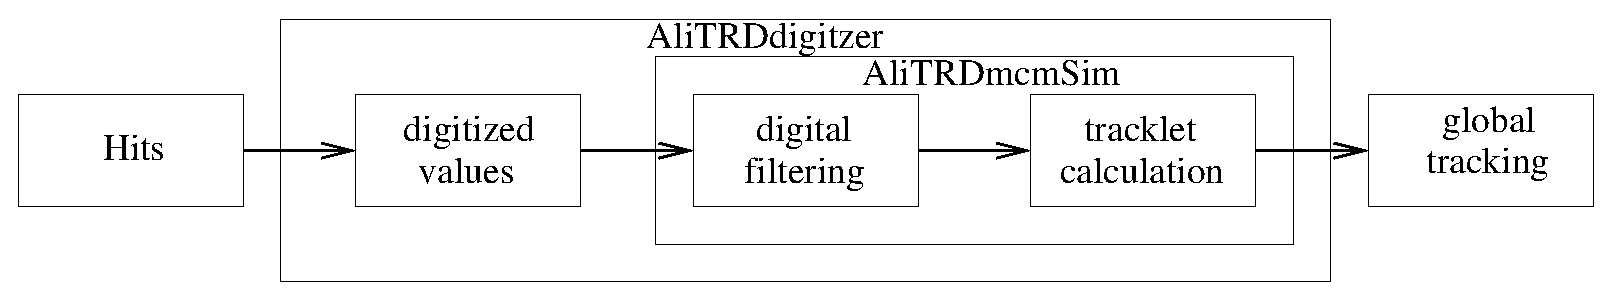
\includegraphics[angle=0,width=0.9\textwidth]{plots/trgsim_ov}
\end{center}
\caption[Trigger simulation overview]{Overview of the trigger
  simulation}
\label{fig:trgsim}
\end{figure}

\subsection{MCM simulation}
The MCM simulation is contained in {\tt AliTRDmcmSim}. This class
mimics the digital part of an MCM. It can be used for the simulation
after digitization has been performed.

Internally, an object of {\tt AliTRDmcmSim} can hold the data of
21~ADC channels both raw and filtered. After the instantiation {\tt
  Init()} has to be called to define the position of the MCM. Then,
the data can be fed using either of the following methods:
\begin{description}
\item[{\tt SetData(Int\_t iadc, Int\_t *adc)}] ~\\ Set the data for the
  given ADC channel {\it iadc} from an array {\it adc} containing the
  data for all timebins.
\item[{\tt SetData(Int\_t iadc, Int\_t it, Int\_t adc)}] ~\\ Set the data for the
  given ADC channel {\it iadc} and timebin {\it it} to the value {\it adc}.
\item[{\tt SetData(AliTRDarrayADC *adcArray)}] ~\\ Set the data for the
  whole MCM from the digits array pointed to by {\it adcArray}.
\item[{\tt LoadMCM(AliRunLoader *rl, Int\_t det, Int\_t rob, Int\_t mcm)}]
  ~\\ This method automatically initializes the MCM for the specified
  location and loads the relevant data via the runloader pointed by
  {\it rl}. 
\end{description}

After loading of the data the processing stages can be run
individually:
\begin{description}
\item[{\tt Filter()}] ~\\ The pedestal, gain and tail cancellation filters
  are run on the currently loaded raw data. The filter settings
  (including bypasses) are used as configured in the TRAP
  (s.~\ref{sec:trapcfg}). The unfiltered raw data is kept such that it
  is possible to rerun Filter(), e.g. with different settings. 
\item[{\tt Tracklet()}] ~\\ The tracklet calculation operates on the
  filtered data (which is identical to the unfiltered data if Filter()
  was not called). First, the hits are calculated and the fit
  registers filled. Subsequently, the straight line fits for the four
  most promising tracklets are calculated. 
\item[{\tt ZSMapping()}] ~\\ This methods performs the zero-suppression
  which can be based on different criteria (to be configured in the
  TRAP). 
\end{description}

The results of the MCM simulation can be accessed in different ways:
\begin{description}
\item[{\tt WriteData(AliTRDarrayADC *digits)}] ~\\ Hereby, the data are
  written to the pointed digits array. It is part of the TRAP
  configuration whether raw or filtered data is written (EBSF). 
\item[{\tt ProduceRawStream(UInt\_t *buf, Int\_t bufsize, UInt\_t
    iEv)}] ~\\ Produce the raw data stream for this MCM as it will
  appear in the raw data of the half-chamber. 
\item[{\tt ProduceTrackletStream(UInt\_t *buf, Int\_t bufsize)}] ~\\
  Produce the raw stream of tracklets as they appear in raw data. 
\item[{\tt StoreTracklets()}] ~\\ The tracklets are stored via the
  runloader. This has to be called explicitly, otherwise the tracklets
  will not be written. 
\end{description}

\subsection{TRAP configuration} 
\label{sec:trapcfg}
The TRAP configuration is kept in {\tt AliTRDtrapConfig} which is
implemented as singleton. After obtaining a pointer to the class by a
call to {\tt AliTRDtrapConfig::Instance()} values can be changed and read by:
\begin{description}
\item[{\tt SetTrapReg(TrapReg\_t reg, Int\_t value, Int\_t det, Int\_t rob,
  Int\_t mcm)}] ~\\ This sets the given TRAP register given as the
  abbreviation from the TRAP manual with preceding 'k' (enum) to the
  given value. If you specify {\it det}, {\it rob} or {\it mcm} the
  values are changed for individual MCMs. Not specified the setting is
  applied globally. 
\item[{\tt GetTrapReg(TrapReg\_t reg, Int\_t det, Int\_t rob, Int\_t mcm)}]
  ~\\ This method gets the current value of the given TRAP
  registers. If the values are set individually for different MCMs you
  have to pass {\it det}, {\it rob} and {\it mcm}. Otherwise, these
  parameters can be omitted. 
\item[{\tt PrintTrapReg(TrapReg\_t reg, Int\_t det, Int\_t rob, Int\_t mcm)}]
  ~\\ It is similar to the preceding method but prints the information
  to stdout. 
\end{description}

The calculated tracklets can be stored by a call to {\tt AliTRDmcmSim::StoreTracklets()}.

\subsection{Tracklet classes}
In order to unify the different sources of tracklets, e.g. real data
or simulation, all implementations of tracklets derive from the
abstract base class {\tt AliTRDtrackletBase}. The following
implementations are currently in use:
\begin{description}
\item[{\tt AliTRDtrackletWord}] ~\\ This class is meant to represent the
  information as really available from the FEE, i.e. only a 32-bit
  word and the information on the detector it was produced on.
\item[{\tt AliTRDtrackletMCM}] ~\\ Tracklets of this type are produced in
  the MCM simulation and contain additional MC information.
\item[{\tt AliTRDtrackletGTU}] This class is used during the GTU tracking
  and contains a pointer to a tracklet and information assigned to it
  during the global tracking.  
\end{description}

\subsection{GTU simulation}

The simulation of the TRD global tracking on tracklets is steered by
AliTRDgtuSim. This class provides all the interface. The following
classes are involved:
\begin{description}
\item[{\tt AliTRDgtuParam}] ~\\ This class contains or generates the relevant
  parameters used for the GTU tracking. 
\item[{\tt AliTRDgtuTMU}] ~\\ This class holds the actual tracking algorithm
  as it runs in one Track Matching Unit (TMU) which corresponds to one
  stack. 
\end{description}

The GTU simulation can be run by calling {\tt
  AliTRDgtuSim::RunGTU(AliLoader *loader, AliESDEvent *esd)} where
{\it loader} points to the TRD loader and {\it esd} to an ESD
event. The latter can be omitted in which case the output is not
written to the ESD. The tracklets are automatically retrieved via the
loader and the found tracks of type {\tt AliTRDtrackGTU} are
internally stored in a tree for which a getter exists to access. If a
pointer to an {\tt AliESDEvent} is given, the tracks are also written
to the ESD (as {\tt AliESDTrdTrack}). For this the method {\tt
  AliTRDtrackGTU::CreateTrdTrack()} is used which creates the {\tt
  AliESDTrdTrack} (with reduced information compared to {\tt
  AliTRDtrackGTU}).

\subsection{CTP interface}

The interface to the central trigger is defined in {\tt
  AliTRDTrigger}. This class is called automatically during simulation
and produces the trigger inputs for TRD (in {\tt
  CreateInputs()}). They are only considered if they are part of the
used trigger configuration (e.g. GRP/CTP/p-p.cfg).

The actual trigger generation has to be contained in {\tt
  Trigger()}. Currently, the GTU simulation is run from here using the
previously calculated tracklets. The generated tracks are stored and
the trigger inputs are propagated to CTP. Which trigger classes make
use of the TRD inputs has to be defined in the trigger configuration. 
%
%%%%%%%%%%%%%%%%%%%%%%%%%%%%%%%%%%%%%%%%%%%%%%%%%%%%%%%%%%%%%%%%%%%%%
\newpage
\setcounter{chapter}{2}
\setcounter{section}{0}    
\Chapter{Reconstruction}\label{REC:}
{\it Author: A.~Bercuci (A.Bercuci@gsi.de)}
\thispagestyle{empty}
%
\section{Raw Data Reading}
%
\section{Cluster Finding}\label{REC:CL:}
%
\subsection[Cluster position reconstruction]{Cluster position reconstruction
\footnote{The procedures described in this section are implemented in the functions 
{\tt AliTRDcluster::GetXloc()}, {\tt AliTRDcluster::GetYloc()},
{\tt AliTRDcluster::GetSX()} and {\tt AliTRDcluster::GetSY()}.}}\label{REC:CL:rphi}
{\it Author: A.~Bercuci (A.Bercuci@gsi.de)}
\\
{\bf Calculation of cluster position in the radial direction} in local chamber 
coordinates (with respect to the anode wire position) is using the following 
parameters:\\
  $t_0$ - calibration aware trigger delay $[\mu s]$\\
  $v_d$ - drift velocity in the detector region of the cluster $[cm/\mu s]$\\
  $z$ - distance to the anode wire [cm]. By default average over the drift cell width\\
  $q$ \& $x_q$ - array of charges and cluster positions from previous clusters in the tracklet [a.u.]

The estimation of the radial position is based on calculating the drift time 
and the drift velocity at the point of estimation. The drift time can be 
estimated according to the expression:
\begin{equation}
t_{drift} = t_{bin} - t_{0} - t_{cause}(x) - t_{TC}(q_{i-1}, q_{i-2}, ...)
\end{equation}
where $t_0$ is the delay of the trigger signal. $t_{cause}$ is the causality 
delay between ionization electrons hitting the anode and the registration of 
the mean signal by the electronics - due to the rising time of the TRF. A 
second order correction here comes from the fact that the time spreading of 
charge at anode is the convolution of TRF with the diffusion and thus 
cross-talk between clusters before and after local clusters changes with drift 
length. $t_{TC}$ is the residual charge from previous (in time) clusters due 
to residual tails after tail cancellation. This tends to push cluster forward 
and depends on the magnitude of their charge.

The drift velocity varies with the drift length (and distance to anode wire) 
as described by cell structure simulation. Thus one, in principle, can calculate 
iteratively the drift length from the expression:
\begin{equation}
x = t_{drift}(x)*v_{drift}(x)
\end{equation}
In practice we use a numerical approach (see {\tt AliTRDcluster::GetXcorr()} 
and Figure \ref{FIG_CLUSTER:Xcorr} left) to correct for anisochronity obtained 
from a MC comparison (see {\tt AliTRDclusterResolution\-::ProcessSigma()} for 
the implementation). Also the calibration of the 0th approximation (no $x$ 
dependence) for $t_{cause}$ is obtained from MC comparisons and is impossible 
to disentangle in real life from trigger delay.
\begin{figure}[htb]
\begin{center}
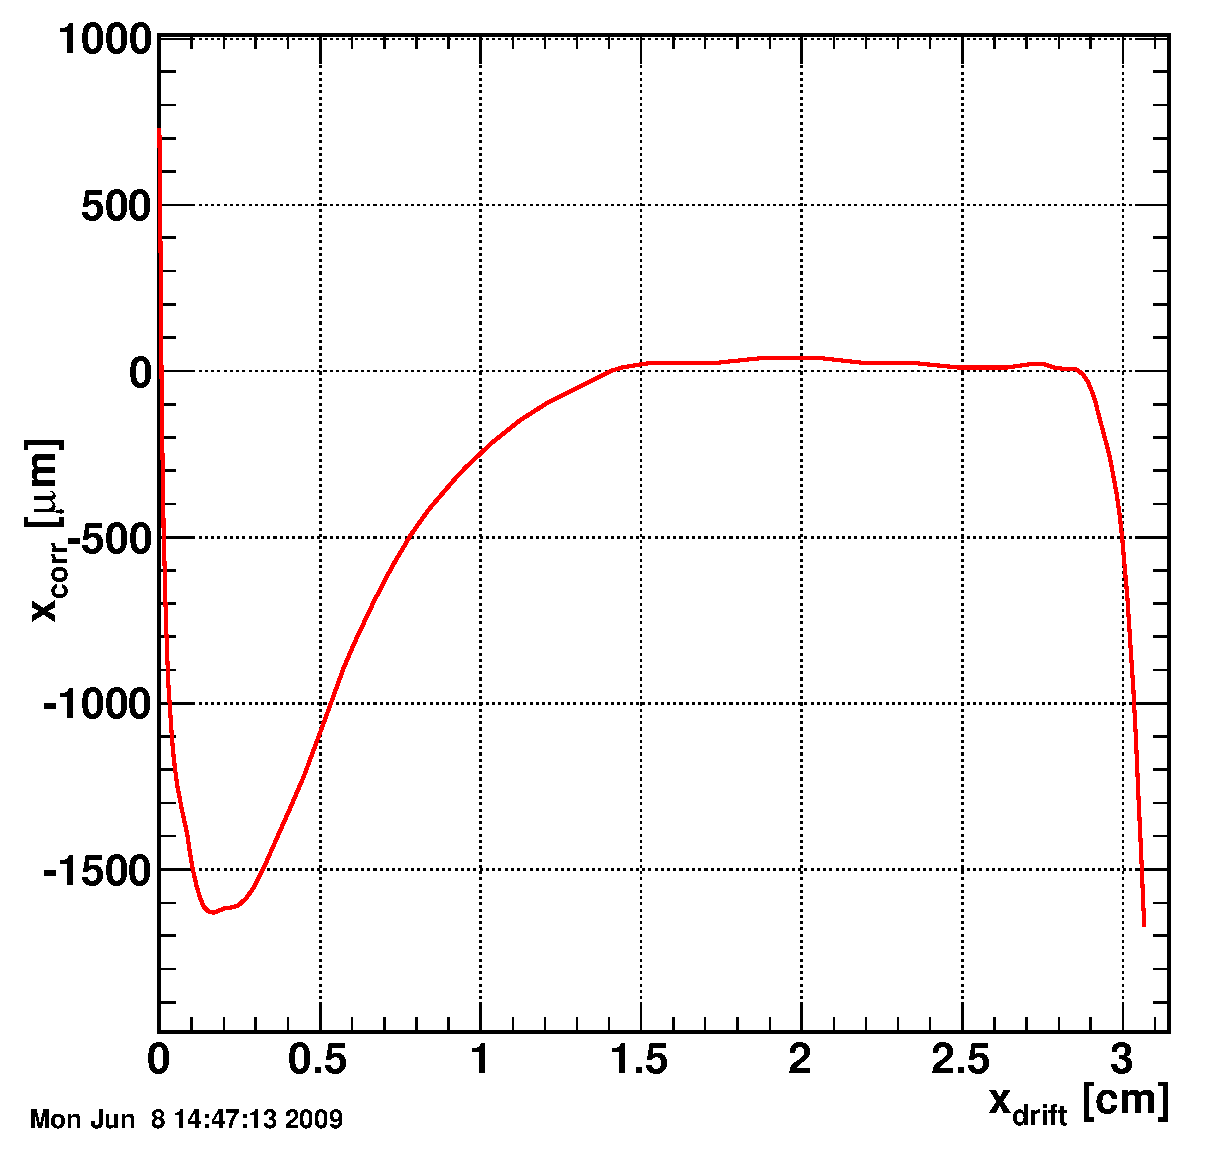
\includegraphics[width=0.48\textwidth]{plots/clusterXcorr.eps}
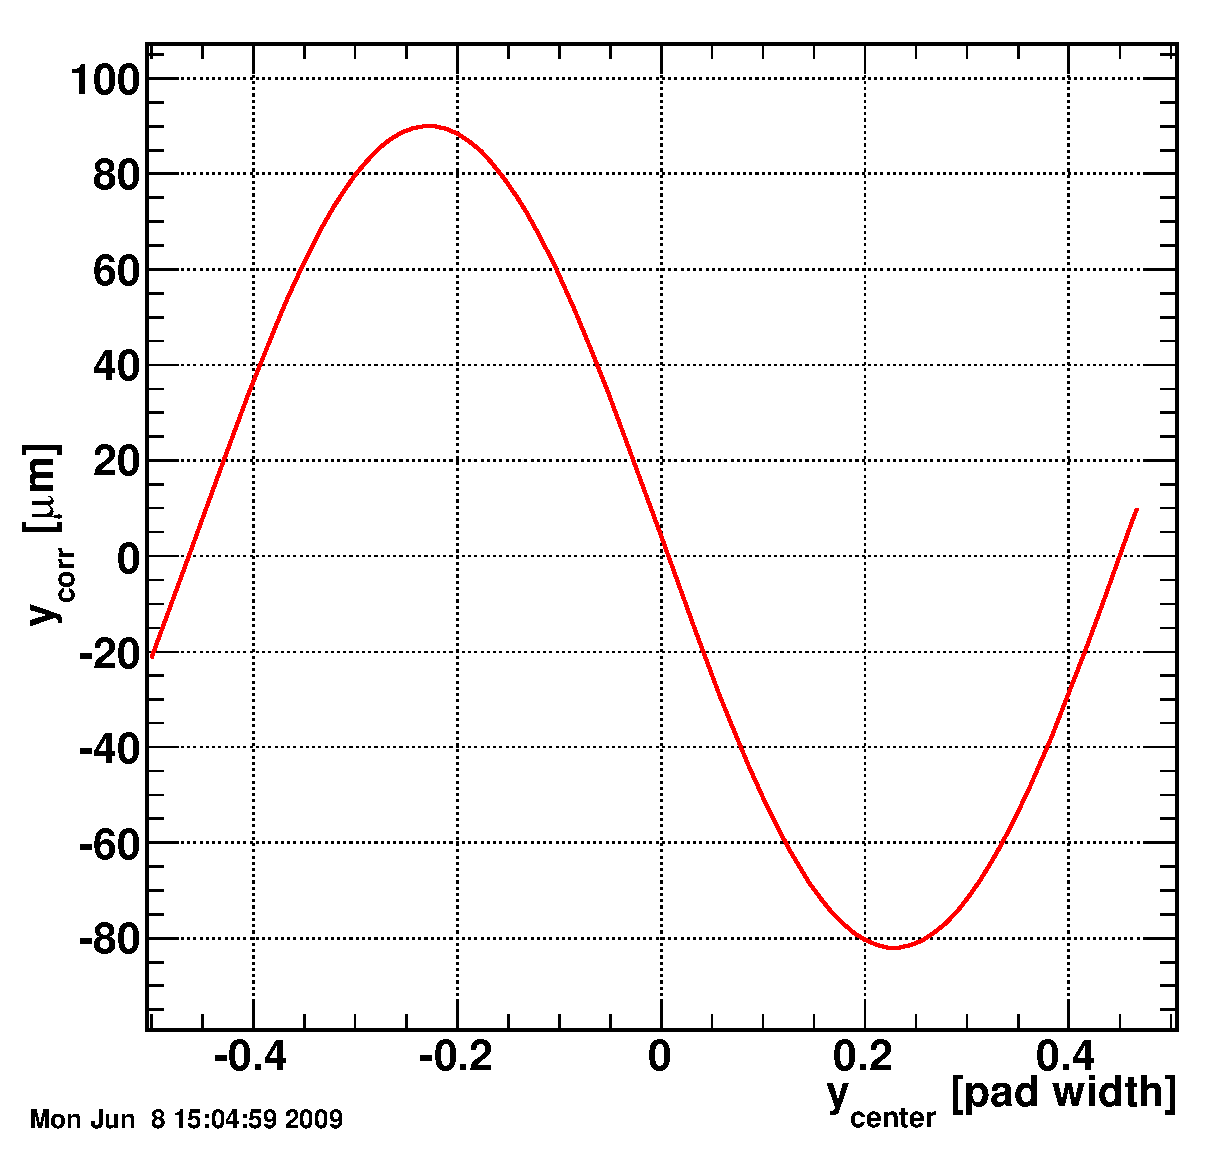
\includegraphics[width=0.48\textwidth]{plots/clusterYcorr.eps}
\end{center}
\caption{
Correction of the radial and $r-\phi$ position of the TRD cluster.}
\label{FIG_CLUSTER:Xcorr}
\end{figure}
\\
\\
For {\bf the calculation of the $r-\phi$ offset} of the cluster from the middle 
of the center pad three methods are implemented:
\begin{itemize}
  \item[-] Center of Gravity (COG) see {\tt AliTRDcluster::GetDYcog()}
  \item[-] Look-up Table (LUT) see {\tt AliTRDcluster::GetDYlut()}
  \item[-] Gaussian shape (GAUS) see {\tt AliTRDcluster::GetDYgauss()}
\end{itemize}
In addition for the case of LUT method position corrections are also applied 
(see {\tt AliTRDcluster\-::GetYcorr()} and Figure \ref{FIG_CLUSTER:Xcorr} right).

One may calculate the $r-\phi$ offset, based on the Gaussian approximation of 
the PRF, from the signals $q_{i-1}$, $q_i$ and $q_{i+1}$ in the 3 adjacent pads 
by:
\begin{equation}
y = \frac{1}{w_{1}+w_{2}} \left[ w_{1} \left( y_{0}-\frac{W}{2}
                                                   +\frac{s^{2}}{W}
                                                    \ln\frac{q_{i}}{q_{i-1}} \right)
                                + w_{2}\left( y_{0}+\frac{W}{2}
                                                   +\frac{s^{2}}{W}
                                                    \ln\frac{q_{i+1}}{q_{i}} \right) \right]
\end{equation}
where $W$ is the pad width, $y_0$ is the position of the middle of the center 
pad and $s^2$ is given by
\begin{equation}
s^{2} = s^{2}_{0} + s^{2}_{diff} (x,B) + \frac{\tan^{2}(\phi-\alpha_{L})*l^{2}}{12}
\end{equation}
with $s_0$ being the PRF for 0 drift and track incidence $\phi$ equal to the Lorentz 
angle $\alpha_L$ and the diffusion term being described by:
\begin{equation}
s_{diff} (x,B) = \frac{D_{L}\sqrt{x}}{1+({\omega\tau}^{2})}
\end{equation}
with $x$ being the drift length. The weights $w_1$ and $w_2$ are taken to be 
$q_{i-1}^2$ and $q_{i+1}^2$ respectively.
\\

\noindent
{\bf Determination of shifts by comparing with MC}
\\

The resolution of the cluster corrected for pad tilt with respect to MC in the 
$r-\phi$ (measuring) plane can be expressed by:
\begin{eqnarray}
\Delta y&=&w - y_{MC}(x_{cl})\\
w &=& y_{cl}^{'} + h*(z_{MC}(x_{cl})-z_{cl})\\
y_{MC}(x_{cl}) &=& y_{0} - dy/dx*x_{cl}\\
z_{MC}(x_{cl}) &=& z_{0} - dz/dx*x_{cl}\\
y_{cl}^{'} &=& y_{cl}-x_{cl}*\tan(\alpha_{L})
\end{eqnarray}
where $x_{cl}$ is the drift length attached to a cluster, $y_{cl}$ is the 
$r-\phi$ coordinate of the cluster measured by charge sharing on adjacent pads 
and $y_0$ and $z_0$ are MC reference points (as example the track references at 
entrance/exit of a chamber). If we suppose that both $r-\phi$ ($y$) and radial 
($x$) coordinate of the clusters are affected by errors we can write
\begin{eqnarray}
x_{cl} &=& x_{cl}^{*} + \delta x\\ 
y_{cl} &=& y_{cl}^{*} + \delta y 
\end{eqnarray} 
where the starred components are the corrected values. Thus by definition the 
following quantity
\begin{equation}
\Delta y^{*}= w^{*} - y_{MC}(x_{cl}^{*})
\end{equation}
has 0 average over all dependency. Using this decomposition we can write:
\begin{equation}\label{EQ_CLUSTER:shift}
<\Delta y>=<\Delta y^{*}> + <\delta x * (dy/dx-h*dz/dx) + \delta y - \delta x 
          * \tan(\alpha_{L})>
\end{equation}
which can be transformed to the following linear dependence:
\begin{equation}
<\Delta y>= <\delta x> * (dy/dx-h*dz/dx) + <\delta y - \delta x * \tan(\alpha_{L})>
\end{equation}
if expressed as function of $dy/dx-h*dz/dx$. Furtheremore this expression can 
be plotted for various clusters i.e. we can explicitely introduce the diffusion 
($x_{cl}$) and drift cell - anisochronity ($z_{cl}$) dependences. From 
plotting this dependence and linear fitting it with:
\begin{equation}
<\Delta y>= a(x_{cl}, z_{cl}) * (dy/dx-h*dz/dx) + b(x_{cl}, z_{cl})
\end{equation}
the systematic shifts will be given by:
\begin{eqnarray}
\delta x (x_{cl}, z_{cl}) &=& a(x_{cl}, z_{cl})\\
\delta y (x_{cl}, z_{cl}) &=& b(x_{cl}, z_{cl}) + a(x_{cl}, z_{cl}) * \tan(\alpha_{L})
\end{eqnarray}
In Figure \ref{FIG_CLUSTER:shift} left there is an example of such dependency. 
\begin{figure}[htb]
\begin{center}
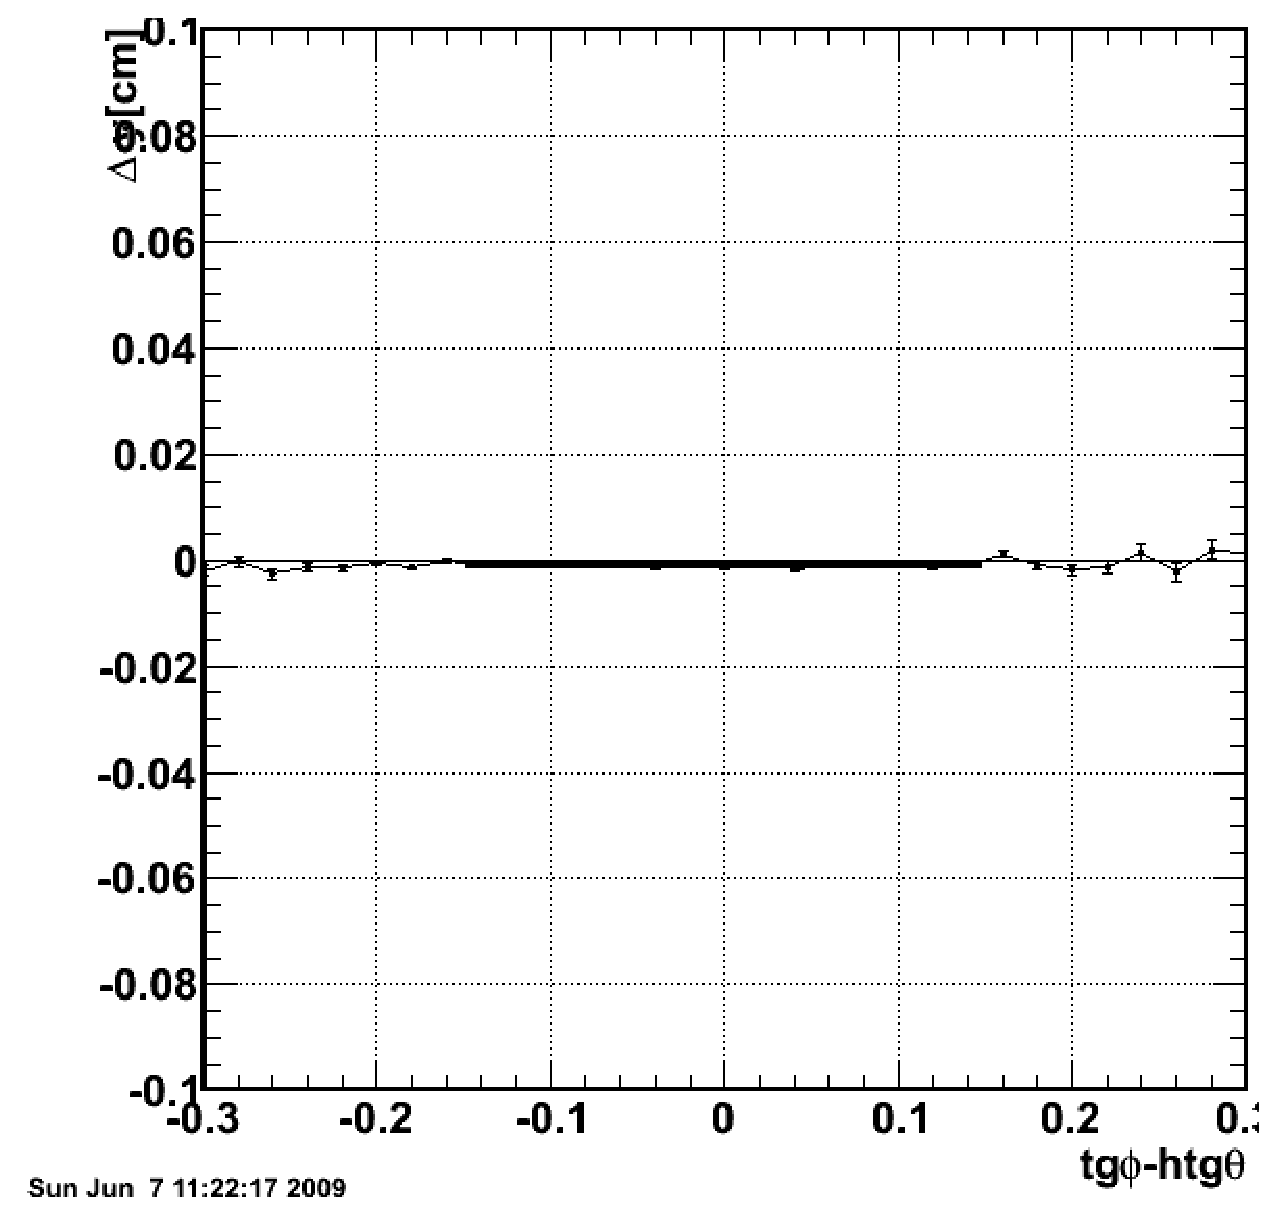
\includegraphics[width=0.48\textwidth]{plots/clusterShiftMethod.eps}
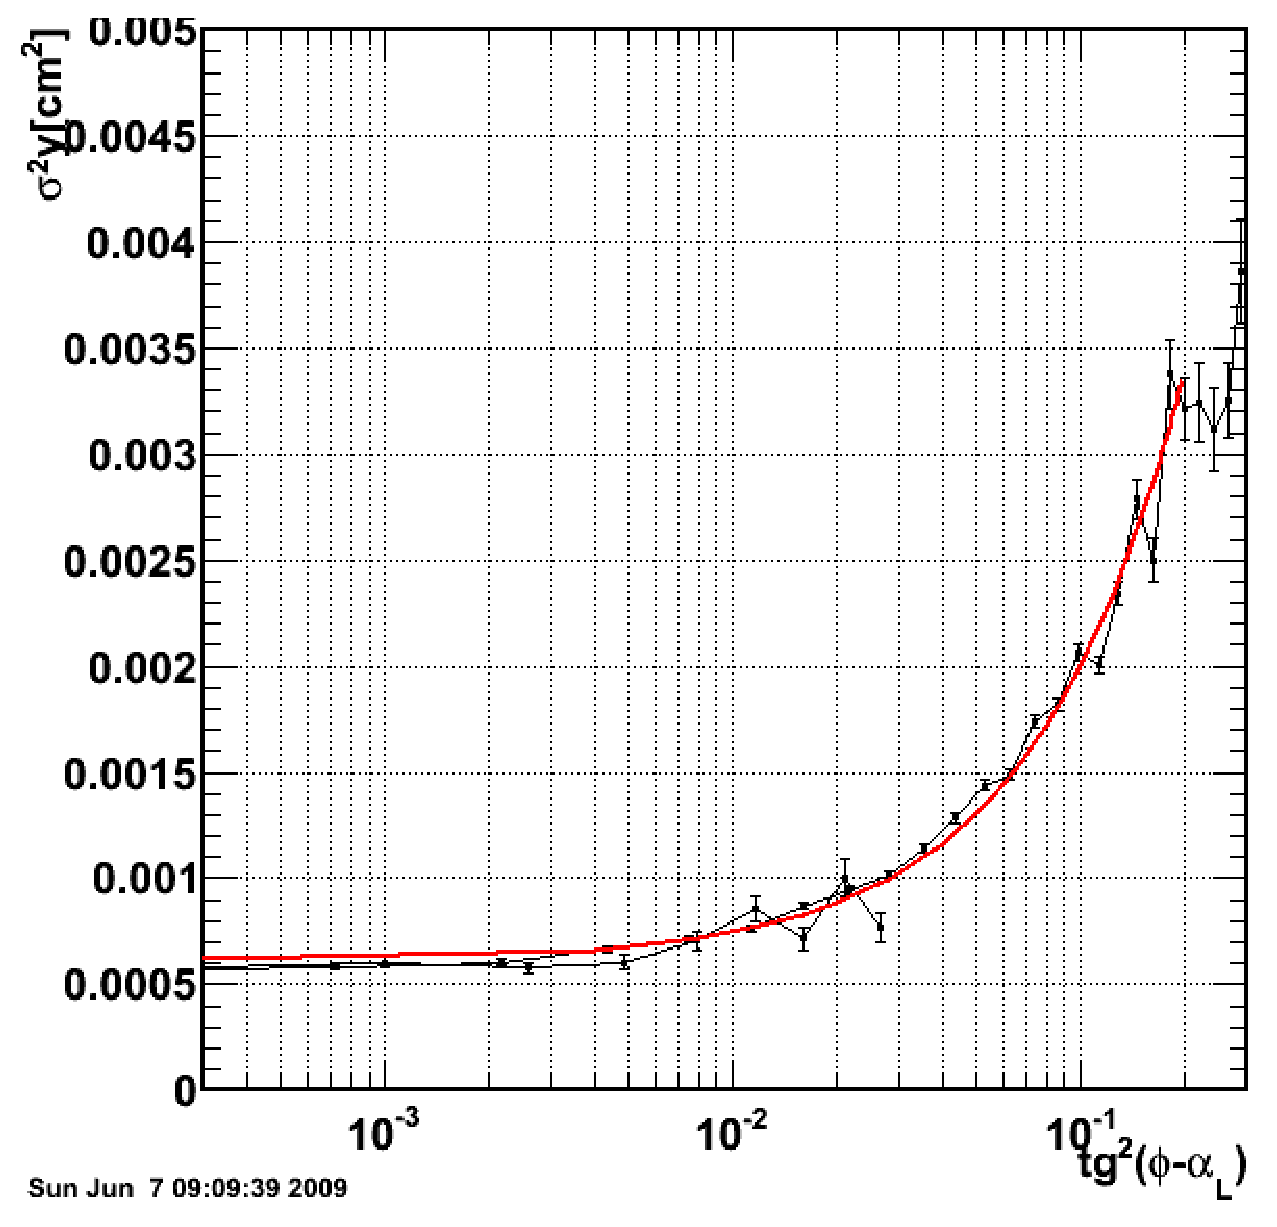
\includegraphics[width=0.48\textwidth]{plots/clusterSigmaMethod.eps}
\end{center}
\caption{
Linear relation to estimate radial and $r-\phi$ cluster shifts and error.}
\label{FIG_CLUSTER:shift}
\end{figure}
\\
\\
The occurance of the radial shift is due to the following conditions:
\begin{itemize}
  \item[-] The approximation of a constant drift velocity over the drift length 
           (larger drift velocities close to the cathode wire plane).
  \item[-] The superposition of charge tails in the amplification region (first 
           clusters appear to be located at the anode wire).
  \item[-] The superposition of charge tails in the drift region (shift towards 
           anode wire).
  \item[-] Diffusion effects which convolute with the TRF thus enlarging it.
  \item[-] Approximate knowledge of the TRF (approximate measuring in test beam 
           conditions).
\end{itemize}
The numerical results for ideal simulations for the radial are displayed in 
Figure \ref{FIG_CLUSTER:Xcorr}.
\\
\\
The representation of $dy=f(y_cen, x_drift| layer, \phi=\tan(\alpha_L))$ can be 
also used to estimate the systematic shift in the $r-\phi$ coordinate resulting 
from an imperfection in the cluster shape parameterization. From 
Eq.~\ref{EQ_CLUSTER:shift} with $\phi=\tan(\alpha_L)$ one gets: 
\begin{eqnarray}
<\Delta y>&=& <\delta x> * (\tan(\alpha_{L})-h*dz/dx) + <\delta y - \delta x * \tan(\alpha_{L})>\\
<\Delta y>(y_{cen})&=& -h*<\delta x>(x_{drift}, q_{cl}) * dz/dx + \delta y(y_{cen}, ...)
\end{eqnarray}
where all dependences are made explicit. This last expression can be used in two ways:
\begin{itemize}
  \item[-] By average on the $dz/dx$ we can determine directly $dy$ (the method 
           implemented here - see Figure \ref{FIG_CLUSTER:Xcorr} right).
  \item[-] By plotting as a function of $dzdx$ one can determine both $dx$ and $dy$ 
           components in an independent method.
\end{itemize}
The occurance of the $r-\phi$ shift is due to the following conditions:
\begin{itemize}
  \item[-] Approximate model for cluster shape (LUT).
  \item[-] Rounding-up problems.
\end{itemize}


\subsection[Cluster error parameterization]{Cluster error parametrization
\footnote{The procedures described in this section are implemented in the functions 
{\tt AliTRDcluster::SetSigmaY2()}, {\tt AliTRDclusterResolution::ProcessCharge()}, 
{\tt AliTRDclusterResolution::ProcessCenterPad()}, 
{\tt AliTRDclusterResolution::ProcessSigma()} and 
{\tt AliTRDclusterResolution::ProcessMean()}.}}\label{REC:CL:error}
{\it Author: A.~Bercuci (A.Bercuci@gsi.de)}
\\

The error of TRD cluster is represented by the variance in the $r-\phi$ and radial 
direction. For the $z$ direction the error is simply given by:
\begin{equation}
\sigma^2_z=L^2_{pad}/12
\end{equation}

The parameters on which the {\bf $r-\phi$ error parameterization} depends are:
\begin{itemize}
  \item[-] $s^2$  - variance due to PRF width for the case of Gauss model. Replaced 
           by parameterization in case of LUT.
  \item[-] $dt$  - transversal diffusion coefficient.
  \item[-] $e \times B$ - tangens of Lorentz angle.
  \item[-] $x$-drift length - with respect to the anode wire.
  \item[-] $z$-offset from the anode wire.
  \item[-] $\tan(p)$ - local tangens of the track momentum azimuthal angle.
\end{itemize}

The ingredients from which the error is computed are:
\begin{itemize}
  \item[-] PRF (charge sharing on adjacent pads)  - see {\tt AliTRDcluster::GetSYprf()}.
  \item[-] Diffusion (dependence with drift length and [2nd order] distance to anode wire) 
           (see {\tt AliTRDcluster::GetSYdrift()}).
  \item[-] Charge of the cluster (complex dependence on gain and tail cancellation) - see 
           ({\tt AliTRD\-cluster::GetSYcharge()}).
  \item[-] Lorentz angle (dependence on the drift length and [2nd order] distance to anode 
           wire) - see {\tt AliTRDcluster::GetSX()}.
  \item[-] Track angle (superposition of charges on the anode wire) 
           (see {\tt AliTRDseedV1::Fit()}).
  \item[-] Projection of radial ($x$) error on $r-\phi$ due to fixed value assumed in 
           tracking for $x$ - see {\tt AliTRDseedV1::Fit()}.
\end{itemize}

The last 2 contributions to cluster error can be estimated only during tracking 
when the track angle is known ($\tan(p)$). For this reason the errors (and 
optional position) of TRD clusters are recalculated during tracking and thus 
clusters attached to tracks might differ from bare clusters.

Taking into account all contributions one can write the the TRD cluster error 
parameterization as:
\begin{equation}\label{EQ_CLUSTER:error}
\sigma_{y}^{2} = (\sigma_{diff}*\rm{Gauss}(0, s_{ly}) + \delta_{\sigma}(q))^{2} 
               + \tan^{2}(\alpha_{L})*\sigma_{x}^{2} 
               + \tan^{2}(\phi-\alpha_{L})*\sigma_{x}^{2}
               + [\tan(\phi-\alpha_{L})*\tan(\alpha_{L})*x]^{2}/12
\end{equation}
From this formula one can deduce that the simplest calibration method for PRF and 
diffusion contributions is by measuring resolution at $B = 0$~T and $\phi = 0$. 
To disentangle further the two remaining contributions one has to represent $s^2$ 
as a function of drift length. 

In the Gaussian model the diffusion contribution can be expressed as:
\begin{equation}
\sigma^{2}_{y} = \sigma^{2}_{PRF} + \frac{x\delta_{t}^{2}}{(1+\tan(\alpha_{L}))^{2}}
\end{equation}
thus resulting the PRF contribution. For the case of the LUT model both contributions 
have to be determined from the fit (see {\tt AliTRDclusterResolution::ProcessCenterPad()} 
for details).
\\

\noindent
{\bf Parameterization with respect to the distance to the middle of the center pad}
\\

If $\phi = \alpha_L$ in Eq.~\ref{EQ_CLUSTER:error}  one gets the following expression:
\begin{equation}\label{EQ_CLUSTER:errorPhiAlpha}
\sigma_{y}^{2} = \sigma_{y}^{2}|_{B=0} + \tan^{2}(\alpha_{L})*\sigma_{x}^{2}
\end{equation}
where we have explicitely marked the remaining term in case of absence of magnetic 
field. Thus one can use the previous equation to estimate $s_y$ for B~=~0 and than 
by comparing in magnetic field conditions one can get the $s_x$. This is a simplified 
method to determine the error parameterization for $s_x$ and $s_y$ as compared to the one 
implemented in {\tt ProcessSigma()}. For more details on cluster error 
parameterization please see also {\tt AliTRDcluster::SetSigmaY2()}.
\\

\noindent
{\bf Parameterization with respect to drift length and distance to the anode wire}
\\

As the $r-\phi$ coordinate is the only one which is measured by the TRD detector we 
have to rely on it to estimate both the radial ($x$) and $r-\phi$ ($y$) errors. This 
method is based on the following assumptions. The measured error in the $y$ 
direction is the sum of the intrinsic contribution of the $r-\phi$ measurement
with the contribution of the radial measurement - because $x$ is not a parameter of 
Alice track model (Kalman).
\begin{equation}
\sigma^{2}|_{y} = \sigma^{2}_{y*} + \sigma^{2}_{x*}   
\end{equation}
In the general case 
\begin{eqnarray}
\sigma^{2}_{y*}& =& \sigma^{2}_{y} + \tan^{2}(\alpha_{L})\sigma^{2}_{x_{drift}}\\   
\sigma^{2}_{x*} &=& \tan^{2}(\phi - \alpha_{L})*(\sigma^{2}_{x_{drift}} 
                 + \sigma^{2}_{x_{0}} + \tan^{2}(\alpha_{L})*x^{2}/12)
\end{eqnarray}
where we have explicitely show the Lorentz angle correction on $y$ and the projection 
of radial component on the $y$ direction through the track angle in the bending plane 
($\phi$). Also we have shown that the radial component in the last equation has two 
terms, the drift and the misalignment ($x_0$). For ideal geometry or known misalignment 
one can solve the equation
\begin{equation}
\sigma^{2}|_{y} = \tan^{2}(\phi - \alpha_{L})*(\sigma^{2}_{x} 
                + \tan^{2}(\alpha_{L})*x^{2}/12)
                + [\sigma^{2}_{y} + \tan^{2}(\alpha_{L})\sigma^{2}_{x}]
\end{equation}
by fitting a straight line:
\begin{equation}
\sigma^{2}|_{y} = a(x_{cl}, z_{cl}) * \tan^{2}(\phi - \alpha_{L}) + b(x_{cl}, z_{cl})
\end{equation}
the error parameterization will be given by:
\begin{eqnarray}
\sigma_{x} (x_{cl}, z_{cl}) &=& \sqrt{a(x_{cl}, z_{cl}) - \tan^{2}(\alpha_{L})*x^{2}/12}\\
\sigma_{y} (x_{cl}, z_{cl}) &=& \sqrt{b(x_{cl}, z_{cl}) - \sigma^{2}_{x} (x_{cl}, z_{cl}) 
                             * \tan^{2}(\alpha_{L})}
\end{eqnarray}
In Figure \ref{FIG_CLUSTER:shift} left, there is an example of such dependency. 

The error parameterization obtained by this method are implemented in the functions 
{\tt AliTRD\-cluster::GetSX()} and {\tt AliTRDcluster::GetSYdrift()}. 

An independent method to determine $s_y$ as a function of drift length (see 
{\tt AliTRDcluster\-Resolution::ProcessCenterPad()}) is to plot cluster resolution as 
a function of drift length at $\phi = \alpha_L$ as seen in 
Eq.~\ref{EQ_CLUSTER:errorPhiAlpha}. Thus one can use directly the previous equation 
to estimate $s_y$ for $B = 0$ and than by comparing in magnetic field conditions one 
can get the $s_x$.

One has to keep in mind that while the first method returns the mean $s_y$ over the 
distance to the middle of center pad ($y_{center}$) distribution the second method 
returns the *STANDARD* value at $y_{center}=0$ (maximum). To recover the standard 
value one has to solve the obvious equation:
\begin{equation}
\sigma_{y}^{STANDARD} = \frac{<\sigma_{y}>}{\int{s exp(s^{2}/\sigma) ds}}
\end{equation}
with "$<s_y>$" being the value calculated in first method and "sigma" the width of 
the $s_y$ distribution calculated in the second.
\\

\noindent
{\bf Parameterization with respect to cluster charge}
\\

In Eq.~\ref{EQ_CLUSTER:errorPhiAlpha} one can explicitely write:
\begin{equation}
\sigma_{y}|_{B=0} = \sigma_{diff}*Gauss(0, s_{ly}) + \delta_{\sigma}(q)
\end{equation}
which further can be simplified to:
\begin{eqnarray}
<\sigma_{y}|_{B=0}>(q) &=& <\sigma_{y}> + \delta_{\sigma}(q)\\
<\sigma_{y}> &=& \int{f(q)\sigma_{y}dq}
\end{eqnarray}
The results for $s_y$ and $f(q)$ are displayed in Fig.~\ref{FIG_CLUSTER:errorCharge}:
\begin{figure}[htb]
\begin{center}
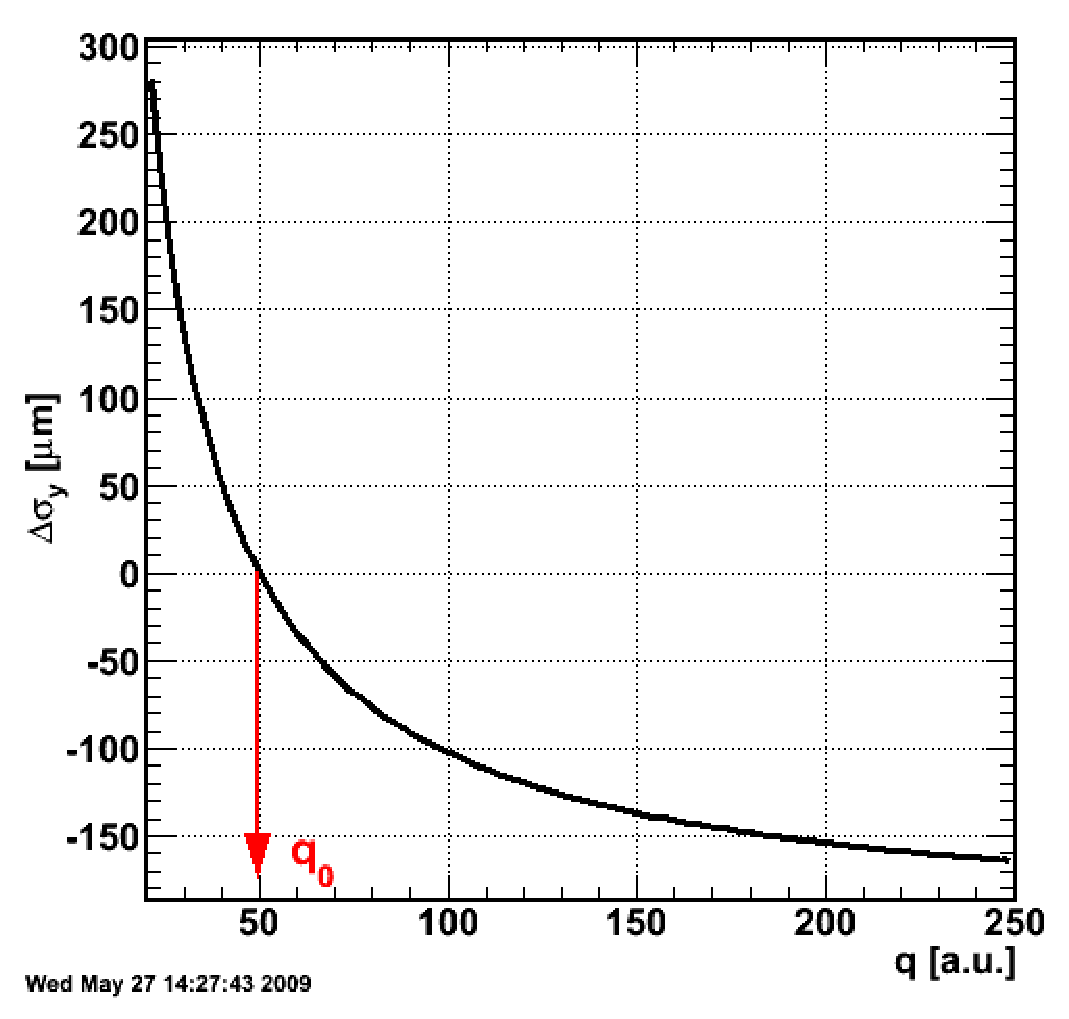
\includegraphics[width=0.48\textwidth]{plots/clusterQerror.eps}
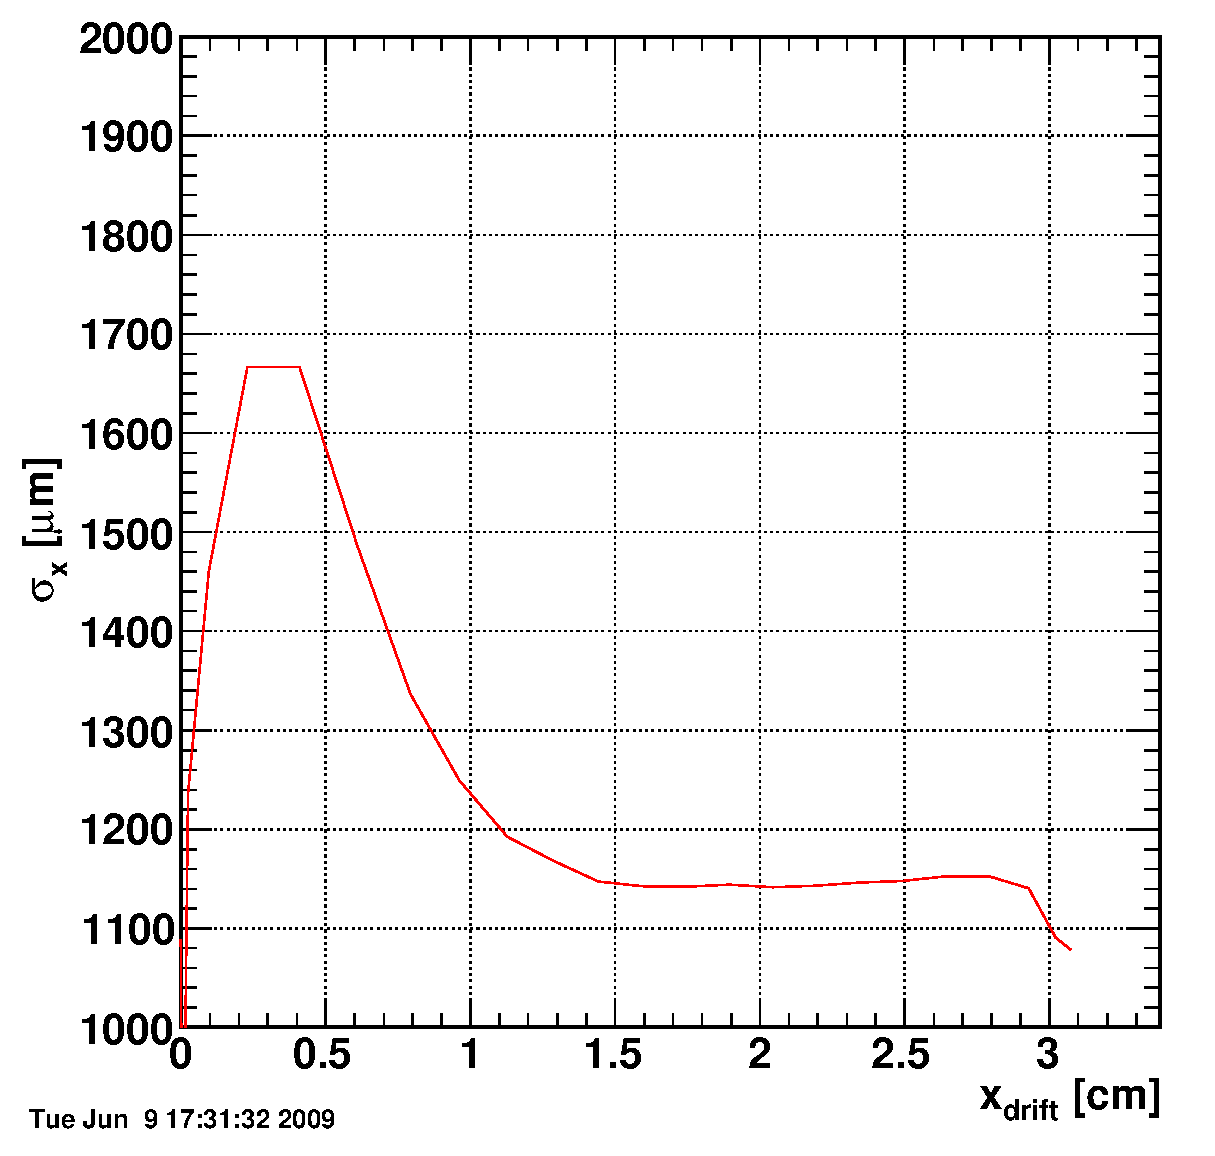
\includegraphics[width=0.48\textwidth]{plots/clusterSX.eps}
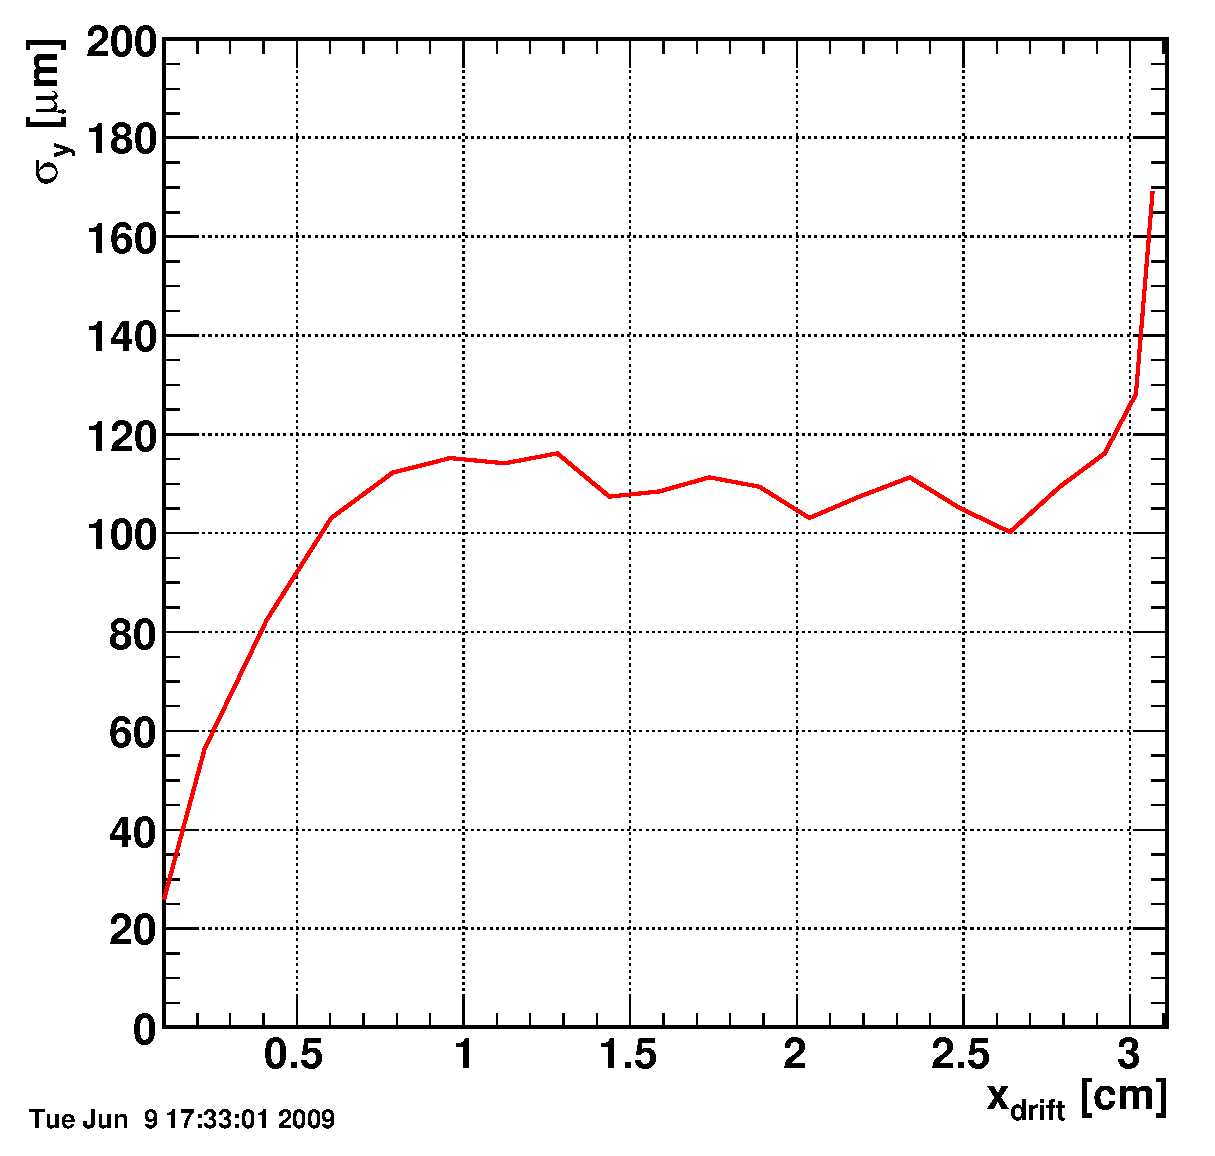
\includegraphics[width=0.48\textwidth]{plots/clusterSY.eps}
\end{center}
\caption{
Cluster error parameterization for different components.}
\label{FIG_CLUSTER:errorCharge}
\end{figure}
The function has to extended to accommodate gain calibration scaling and errors.

%
\setcounter{footnote}{0}
\section{The TRD tracklet}\label{REC:Tracklet:}
{\it Author: A.~Bercuci (A.Bercuci@gsi.de)}\\

\noindent
The tracking in TRD can be done in two major ways:
\begin{itemize}
\item[-] Track prolongation from TPC.
\item[-] Stand alone track finding.
\end{itemize}
The first mode is the main tracking mode for all barrel tracks while the second 
is used to peak-up track segments fully contained in the TRD fiducial volume 
like conversions. Another feature of the TRD tracking besides the relative high 
thickness (conversions) is the spatial correlation of the signals in the radial 
direction due to residual tails in the cluster signals. This feature asked for 
an intermediate step between clusters and tracks, the tracklets. The TRD 
tracklets are linear fits of the clusters from one chamber. They are implemented 
in the class {\tt AliTRDseedV1} and they represent the core of the TRD offline 
reconstruction. In the following the tracklets will be described independently 
of the framework in which they are living (tracking) in the sections 
\ref{REC:Tracking:TrackletAttach}, \ref{REC:Tracking:TrackletFit} and 
\ref{REC:Tracking:TrackletErrors} and than their usage will be outlined in the 
barrel (section \ref{REC:Tracking:Propagate}) and stand alone tracking (section 
\ref{REC:Tracking:Clusters2TracksStack}).

\subsection[Tracklet building]{Tracklet building - Attaching clusters to tracklet
\footnote{The procedures described in this section are implemented in the function 
{\tt AliTRDseedV1::AttachClusters()}.}}\label{REC:Tracking:TrackletAttach}

Projective algorithm to attach clusters to seeding tracks. The following steps are 
performed:
\begin{enumerate}
\item[-] Collapse $x$ coordinate for the full detector along track direction $dy dx$.
\item[-] Truncated mean on $y$ ($r-\phi$) direction.
\item[-] Purge clusters.
\item[-] Truncated mean on $z$ direction.
\item[-] Purge clusters.
\end{enumerate}
Optionally one can use the $z$, $dz/dx$ information from the seeding track to 
correct for tilting.
	
We start up by defining the track direction in the $xy$ plane and roads. The 
roads are calculated based on tracking information (variance in the $r-\phi$ 
direction) and estimated variance of the standard clusters (see 
{\tt AliTRDcluster::SetSigmaY2()}) corrected for tilt (see {\tt GetCovAt()}). 
From this the road is:
\begin{eqnarray}
r_{y} &=& 3*\sqrt{12*(\sigma^{2}_{Trk}(y) + \frac{\sigma^{2}_{cl}(y) 
+ \tan^{2}(\alpha_{L})\sigma^{2}_{cl}(z)}{1+\tan^{2}(\alpha_{L})})}\\
r_{z} &= &1.5*L_{pad}
\end{eqnarray}

\subsection[Tracklet fitting]{Tracklet fitting\footnote{The procedures described in this 
section are implemented in the function 
{\tt AliTRDseedV1::Fit()}.}}\label{REC:Tracking:TrackletFit}

\noindent
{\bf Fit in the $xy$ plane}
\\

The fit is performed to estimate the $y$ position of the tracklet and the track 
angle in the bending plane. The clusters are represented in the chamber coordinate 
system (with respect to the anode wire - see 
{\tt AliTRDtrackerV1::FollowBackProlongation()} on how this is set). The $x$ and $y$ 
position of the cluster and also their variances are known from clusterizer level 
(see {\tt AliTRDcluster::GetXloc()}, 
{\tt AliTRDcluster::GetYloc()}, {\tt AliTRDcluster::GetSX()} and \\
{\tt AliTRDcluster::GetSY()}). If a Gaussian approximation is used to calculate 
$y$ coordinate of the cluster the position is recalculated taking into account the 
track angle.

Since errors are calculated only in the $y$ directions, radial errors ($x$ direction) 
are mapped to $y$ by projection i.e.
\begin{equation}
\sigma_{x|y} = \tan(\phi) \sigma_{x}
\end{equation}
and also by the Lorentz angle correction.
\\

\noindent
{\bf Fit in the xz plane}
\\

The "fit" is performed to estimate the radial position ($x$ direction) where pad 
row cross happens. If no pad row crossing the $z$ position is taken from geometry 
and radial position is taken from the $xy$ fit (see below).

There are two methods to estimate the radial position of the pad row cross:\\
1. leading cluster radial position: Here the lower part of the tracklet is 
considered and the last cluster registered (at radial $x_{0}$) on this segment 
is chosen to mark the pad row crossing. The error of the $z$ estimate is given by :
\begin{equation}
\sigma_{z} = \tan(\theta) \Delta x_{x_{0}}/\sqrt{12}
\end{equation}
The systematic errors for this estimation are generated by the following sources:
  - no charge sharing between pad rows is considered (sharp cross)
  - missing cluster at row cross (noise peak-up, under-threshold signal etc.).
\\
2. charge fit over the crossing point: Here the full energy deposit along 
the tracklet is considered to estimate the position of the crossing by a fit 
in the $qx$ plane. The errors in the $q$ directions are parameterized as 
$\sigma_q = q^2$. The systematic errors for this estimation are generated by the 
following sources:
\begin{itemize}
\item[-] No general model for the $qx$ dependence.
\item[-] Physical fluctuations of the charge deposit.
\item[-] Gain calibration dependence.
\end{itemize}

\noindent
{\bf Estimation of the radial position of the tracklet}\\

For pad row cross the radial position is taken from the $xz$ fit (see above). 
Otherwise it is taken as the interpolation point of the tracklet i.e. the 
point where the error in $y$ of the fit is minimum. The error in the $y$ 
direction of the tracklet is (see {\tt AliTRDseedV1::GetCovAt()}):
\begin{equation}
\sigma_{y} = \sigma^{2}_{y_{0}} + 2x\:cov(y_{0}, dy/dx) + \sigma^{2}_{dy/dx}
\end{equation}
and thus the radial position is:
\begin{equation}
x = - cov(y_{0}, dy/dx)/\sigma^{2}_{dy/dx}
\end{equation}
\\

\noindent
{\bf Estimation of tracklet position error}\\ 

The error in $y$ direction is the error of the linear fit at the radial 
position of the tracklet while in the $z$ direction is given by the cluster 
error or pad row cross error. In case of no pad row cross this is given by:
\begin{eqnarray}
\sigma_{y} &=& \sigma^{2}_{y_{0}} - 2cov^{2}(y_{0}, dy/dx)/\sigma^{2}_{dy/dx} 
            + \sigma^{2}_{dy/dx}\\
\sigma_{z} &=& L_{pad}/\sqrt{12}
\end{eqnarray}
For pad row cross the full error is calculated at the radial position of the 
crossing (see above) and the error in $z$ by the width of the crossing region - 
being a matter of parameterization. 
\begin{equation}
\sigma_{z} = \tan(\theta) \Delta x_{x_{0}}/\sqrt{12}
\end{equation}
In case of no tilt correction (default in the barrel tracking) the tilt is 
taken into account by the rotation of the covariance matrix. See 
{\tt AliTRDseedV1::GetCovAt()} or \ref{REC:Tracking:TrackletErrors} for details.

\subsection[Tracklet errors]{Tracklet errors\footnote{The procedures described in this 
section are implemented in the function 
{\tt AliTRDseedV1::GetCovAt()}.}}\label{REC:Tracking:TrackletErrors}

In general, for the linear transformation
\begin{equation}
Y = T_{x} X^{T}
\end{equation}
the error propagation has the general form
\begin{equation}
C_{Y} = T_{x} C_{X} T_{x}^{T} 
\end{equation}
We apply this formula 2 times. First to calculate the covariance of the tracklet 
at point $x$ we consider: 
\begin{eqnarray}
T_{x} &=& (1\; x)\\ 
X&=&(y0\; dy/dx)\\
C_{X}&=&
  \left( \begin{array}{cc}
    Var(y0) & Cov(y0, dy/dx)\\
    Cov(y0, dy/dx) & Var(dy/dx) 
  \end{array} \right)
\end{eqnarray}
and secondly to take into account the tilt angle
\begin{eqnarray}
T_{\alpha}& = &
  \left( \begin{array}{cc}
    cos(\alpha)&sin(\alpha)\\
    -sin(\alpha)& cos(\alpha)
  \end{array} \right)\\
X&=&(y\; z)\\ 
C_{X}&=&
  \left( \begin{array}{cc}
    Var(y) &0\\
    0 &Var(z) 
  \end{array} \right)
\end{eqnarray}
using simple trigonometric one can write for this last case
\begin{equation}
C_{Y}=\frac{1}{1+\tan^{2}\alpha} 
  \left( \begin{array}{cc}
    \sigma_{y}^{2}+\tan^{2}(\alpha)\sigma_{z}^{2} &  
    \tan(\alpha)(\sigma_{z}^{2}-\sigma_{y}^{2})\\
    \tan(\alpha)(\sigma_{z}^{2}-\sigma_{y}^{2}) & 
    \sigma_{z}^{2}+\tan^{2}(\alpha)\sigma_{y}^{2}
  \end{array} \right)
\end{equation}
which can be approximated for small alphas (2 deg) with
\begin{equation}
C_{Y}=
  \left( \begin{array}{cc}
    \sigma_{y}^{2} & (\sigma_{z}^{2}-\sigma_{y}^{2})\tan(\alpha)\\
    ((\sigma_{z}^{2}-\sigma_{y}^{2})\tan(\alpha) & \sigma_{z}^{2} 
  \end{array} \right)
\end{equation}
before applying the tilt rotation we also apply systematic uncertainties 
to the tracklet position which can be tuned from outside via the 
{\tt AliTRDrecoParam::SetSysCovMatrix()}. They might account for extra 
misalignment/miscalibration uncertainties. 

\subsection[Tracklet dE/dx]{Energy loss calculations\footnote{The procedures 
described in this section are implemented in the function 
{\tt AliTRDseedV1::CookdEdx()} and 
{\tt AliTRDseedV1::GetdQdl()}.}}\label{REC:Tracking:TrackletdEdx}

Using the linear approximation of the track inside one TRD chamber (TRD tracklet) 
the charge per unit length can be written as:
\begin{equation}
\frac{dq}{dl}(x) = \frac{q_{c}}{dx(x) 
                 * \sqrt{1 + (\frac{dy}{dx})^{2}_{fit} + (\frac{dz}{dx})^{2}_{ref}}}
\end{equation}
where $q_c$ is the total charge collected in the current time bin and $dx$ is the length 
of the time bin (see Fig.~\ref{FIG_TRACKLET:dEdx} right). The representation of charge 
deposit used for PID differs thus in principle from the measured $dQ/dt$ distribution 
(see Fig.~\ref{FIG_TRACKLET:dEdx} left) 
\begin{figure}[htb]
\begin{center}
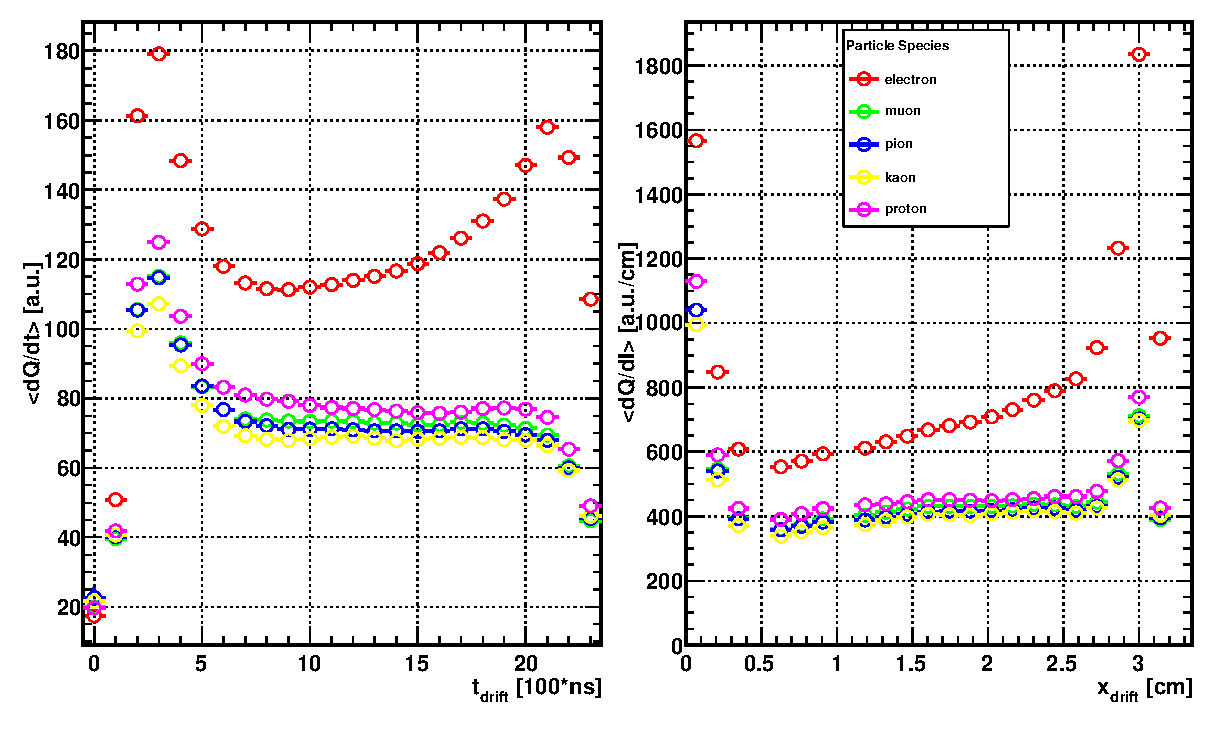
\includegraphics[width=0.88\textwidth, height=0.45\textwidth]{plots/trackletDQDT.eps}
\end{center}
\caption{
Energy loss measurement on the tracklet as a function of drift time [left] and 
respectively drift length [right] for different particle species.}
\label{FIG_TRACKLET:dEdx}
\end{figure} 
The following correction are applied:
\begin{itemize}
\item[-] Charge: pad row cross corrections [diffusion and TRF asymmetry] TODO.
\item[-] $dx$: anisochronity.
\end{itemize}
Due to the anisochronity of the TRD detector drift velocity varies as function of 
drift length and distance to the anode wire. Thus 
\begin{eqnarray}
dx(x) &=& dx(\inf) + \delta_x(x,z)\\ 
      &=& dt*v_d^{\inf} + \delta_x(x,z) 
\end{eqnarray}
the dependence of $\delta_x$ can be found in Fig.~\ref{FIG_CLUSTER:Xcorr}.

\subsection[Tracklet PID]{Particle identification\footnote{The procedures described 
in this section are implemented in the function {\tt AliTRDtrackV1::CookPID()} and 
{\tt AliTRDseedV1::CookPID()}.}}\label{REC:Tracking:TrackletPID}

Retrieve the PID probabilities for $e^\pm$, $\mu^\pm$, $K^\pm$, $\pi^\pm$ and $p^\pm$ 
from the OCDB according to tracklet information:
\begin{itemize}
\item[-] Estimated momentum at tracklet reference point.
\item[-] $dE/dx$ measurements.
\item[-] Tracklet length.
\item[-] TRD layer.
\end{itemize}
According to the steering settings specified in the reconstruction one of the 
following methods are used.
\begin{itemize}
\item[-] Neural Network [default] - option "nn".
\item[-] 2D Likelihood - option "!nn".
\end{itemize}
\begin{figure}[htb]
\begin{center}
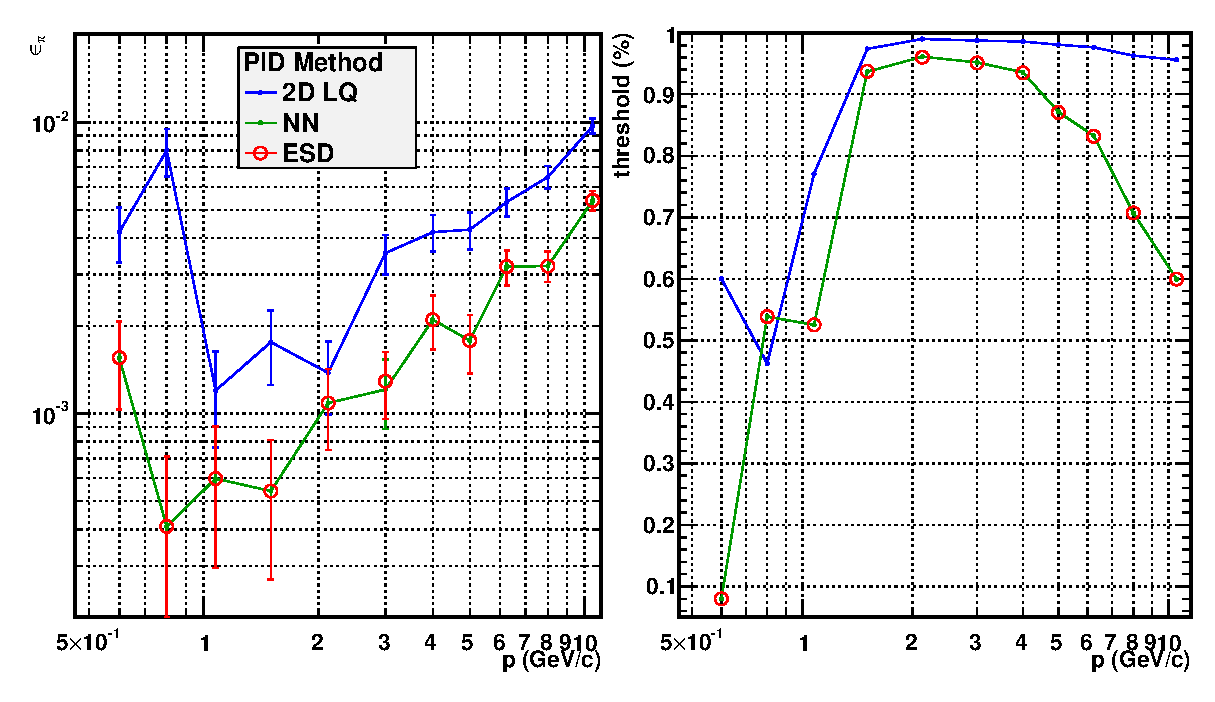
\includegraphics[width=0.88\textwidth, height=0.45\textwidth]{plots/trackPID.eps}
\end{center}
\caption{
Pion efficiency capability of the TRD for tracks with 6 tracklets as a function of 
momentum [left] and the corresponding threshold value for selecting $90\%$ of 
electrons [right] for the two methods used.}
\label{FIG_TRACK:PID}
\end{figure}

At track level the PID information is calculated by delegating the function of 
the tracklets. The number of tracklets used is also computed. The tracklet 
information are considered independent. For the moment no global track measurement 
of PID is performed as for example to estimate bremsstrahlung probability based on 
global $\chi^2$ of the track. The status bit {\tt AliESDtrack::kTRDpid} is set 
during the call of {\tt AliTRDtrackV1::UpdateESDtrack()}. The PID performance of 
the TRD for tracks with 6 tacklets is displayed in Fig.~\ref{FIG_TRACK:PID}. 
\\

\setcounter{footnote}{0}
\section{Tracking}\label{REC:Tracking:}
{\it Author: A.~Bercuci (A.Bercuci@gsi.de)}\\

The tracking procedures in TRD are responsible to attach clusters to tracks 
and to estimate/update the track parameters accordingly. The main class involved 
in this procedure is {\tt AliTRDtrackerV1} and the helper classes {\tt AliTRDcluster}, 
{\tt AliTRDseedV1} and {\tt AliTRDtrackV1}.  Additionally, information from 
{\tt AliTRDrecoParam} is mandatory to select the proper setup of the reconstruction.
\\

\subsection[Track propagation barrel]{Track propagation in barrel tracking\footnote{The 
procedures described in this section are implemented in the function 
{\tt AliTRDtrackerV1::PropagateBack()}.}}\label{REC:Tracking:Propagate}

Propagate the ESD tracks from TPC to TOF detectors and building of the TRD track. For 
building a TRD track an ESD track is used as seed. The informations obtained on the TRD 
track (measured points, covariance, PID, etc.) are than used to update the corresponding 
ESD track. Each track seed is first propagated to the geometrical limit of the TRD 
detector. Its prolongation is searched in the TRD and if corresponding clusters are found 
tracklets are constructed out of them (see {\tt AliTRDseedV1::AttachClusters()}) and the 
track is updated. Otherwise the ESD track is left unchanged.

The following steps are performed:
\begin{itemize}
\item[1.] Selection of tracks based on the variance in the $y-z$ plane.
\item[2.] Propagation to the geometrical limit of the TRD volume. If track 
          propagation fails the {\tt AliESDtrack::kTRDStop} is set.
\item[3.] Prolongation inside the fiducial volume (see 
          {\tt AliTRDtrackerV1::FollowBackProlonga\-tion()}) and marking
          the following status bits:
          \begin{center}
          \begin{tabular}{|l|l|}  \hline
          {\tt AliESDtrack::kTRDin}     & Tracks enters the TRD fiducial volume.  \\ \hline
          {\tt AliESDtrack::kTRDStop}   & Tracks fails propagation.               \\ \hline
          {\tt AliESDtrack::kTRDbackup} & Tracks fulfills the $\chi^{2}$ 
                                          conditions and qualifies for refitting. \\ \hline
          \end{tabular}
          \end{center}
\item[4.] Writting to friends, PID, MC label, quality etc. Setting the status bit 
          {\tt AliESDtrack::kTRDout}.
\item[5.] Propagation to TOF. If track propagation fails the {\tt AliESDtrack::kTRDStop} 
          is set.
\end{itemize}


\noindent
{\bf TRD Tracklet initialization and Kalman fit}\footnote{The procedures 
described in this section are implemented in the function 
{\tt AliTRDtrackerV1::FollowBackProlongation()}.}
\\

Starting from the arbitrary radial position of the track this is
extrapolated through the 6 TRD layers. The following steps
are being performed for each layer:
\begin{itemize}
\item[1.] Propagate track to the entrance of the next chamber:
  \begin{itemize}
  \item[-] Get chamber limits in the radial direction.
  \item[-] Check crossing sectors.
  \item[-] Check track inclination.
  \item[-] Check track prolongation against boundary conditions (see exclusion 
           boundaries on {\tt AliTRDgeometry::IsOnBoundary()}).
  \end{itemize}
\item[2.] Build tracklet (see {\tt AliTRDseed::AttachClusters()} for details) for 
          this layer if needed. If only the Kalman filter is needed and tracklets 
          are already linked to the track this step is skipped.
\item[3.] Fit tracklet using the information from the Kalman filter.
\item[4.] Propagate and update track at reference radial position of the tracklet.
\item[5.] Register tracklet with the tracker and track. Update pulls monitoring.
\end{itemize}

During the propagation a bit map is filled detailing the status of the track in 
each TRD chamber.
\begin{center}
\begin{tabular}{|l|l|}  \hline
{\tt AliTRDtrackV1::kProlongation} & Track prolongation failed.                   \\ \hline
{\tt AliTRDtrackV1::kPropagation}  & Track prolongation failed.                   \\ \hline
{\tt AliTRDtrackV1::kAdjustSector} & Failed during sector crossing.               \\ \hline
{\tt AliTRDtrackV1::kSnp}          & Too large bending.                           \\ \hline
{\tt AliTRDtrackV1::kTrackletInit} & Fail to initialize tracklet.                 \\ \hline
{\tt AliTRDtrackV1::kUpdate}       & Fail to attach clusters or fit the tracklet. \\ \hline
{\tt AliTRDtrackV1::kUnknown}      & Anything which is not covered before.        \\ \hline
\end{tabular}
\end{center}
By default the status of the track before first TRD update is saved. 

\subsection[Stand alone track finding]{Stand alone track finding\footnote{The procedures 
described in this section are implemented in the function 
{\tt AliTRDtrackerV1::Clusters2TracksStack()}.}}\label{REC:Tracking:Clusters2TracksStack}

Seeding tracklets and build candidate TRD tracks. The procedure is used during 
barrel tracking to account for tracks which are either missed by TPC prolongation 
or are conversions inside the TRD volume. For stand alone tracking the procedure 
is used to estimate all tracks measured by TRD. 
\\

\noindent
{\bf TRD track finding}\footnote{The procedures described in this section 
are implemented in the function {\tt AliTRDtrackerV1::MakeSeeds()}.}
\\

The following steps are performed:
\begin{itemize}
\item[1.] Build seeding layers by collapsing all time bins from each of the four 
          seeding chambers along the radial coordinate. See 
          {\tt AliTRDtrackingChamber::GetSeedingLayer()} for details. The chambers 
          selection for seeding is described in 
          {\tt AliTRDtrackerV1::Clusters2\-TracksStack()}.
\item[2.] By using the seeding clusters from the seeding layer (step 1) build 
          combinatorics using the following algorithm:
  \begin{itemize}
  \item[-] For each seeding cluster in the lower seeding layer find.
  \item[-] All seeding clusters in the upper seeding layer inside a road defined by 
           a given $\phi$ angle. The angle is calculated on the minimum \pt\ of tracks 
           from the main vertex, accessible by the stand alone tracker.
  \item[-] For each pair of two extreme seeding clusters select middle upper cluster 
           using roads defined externally by the reco params.
  \item[-] Select last seeding cluster as the nearest to the linear approximation of 
           the track described by the first three seeding clusters. The implementation 
           of the road calculation and cluster selection can be found in the functions 
           {\tt AliTRDchamberTimeBin::Build\-Cond()} and 
           {\tt AliTRDchamberTimeBin::GetClusters()}.
  \end{itemize}
\item[3.] Helix fit to the set of eeding clusters 
          (see {\tt AliTRDtrackerFitter::FitRieman(AliTRD\-cluster**)}). No tilt 
          correction is performed at this level 
\item[4.] Initialize seeding tracklets in the seeding chambers.
\item[5.] {\bf Filter 0:} $\chi^{2}$ cut on the $y$ and $z$ directions. The threshold is 
          set externally by the reco params.
\item[6.] Attach (true) clusters to seeding tracklets 
          (see {\tt AliTRDseedV1::AttachClusters()}) and fit tracklet 
          (see {\tt AliTRDseedV1::Fit()}). The number of used clusters used by current 
          seeds should not exceed ... (25).
\item[7.] {\bf Filter 1:} Check if all 4 seeding tracklets are correctly constructed.
\item[8.] Helix fit to the clusters from the seeding tracklets with tilt correction. 
          Refit tracklets using the new approximation of the track. The model of the 
          Riemann tilt fit is based on solving simultaneously the equations:
          \begin{eqnarray}
          R^{2} &=& (x-x_{0})^{2} + (y^{*}-y_{0})^{2}\\
          y^{*} &=& y - \tan(h)(z - z_{t})\\
          z_{t} &=& z_{0}+dzdx*(x-x_{r})
          \end{eqnarray}
          with $(x, y, z)$ the coordinate of the cluster, $(x_0, y_0, z_0)$ the 
          coordinate of the center of the Riemann circle, $R$ its radius, $x_r$ a 
          constant reference radial position in the middle of the TRD stack and $dzdx$ 
          the slope of the track in the $x-z$ plane. Using the following transformations
          \begin{eqnarray}
          t &=& 1 / (x^{2} + y^{2})\\
          u &=& 2 * x * t\\
          v &=& 2 * \tan(h) * t\\
          w &=& 2 * \tan(h) * (x - x_{r}) * t
          \end{eqnarray}
          one gets the following linear equation
          \begin{equation}
          a + b * u + c * t + d * v  + e * w = 2 * (y + \tan(h) * z) * t
          \end{equation}
          where the coefficients have the following meaning 
          \begin{eqnarray}
          a &=& -1/y_{0}\\
          b &=& x_{0}/y_{0}\\
          c &=& (R^{2} -x_{0}^{2} - y_{0}^{2})/y_{0}\\
          d &=& z_{0}\\
          e &=& dz/dx
          \end{eqnarray}
          The error calculation for the free term is thus
          \begin{equation}
          \sigma = 2 * \sqrt{\sigma^{2}_{y}(tilt\ corr ...) 
                 + \tan^{2}(h) * \sigma^{2}_{z}} * t
          \end{equation}
          From this simple model one can compute $\chi^2$ estimates and a rough 
          approximation of $1/p_t$ from the curvature according to the formula:
          \begin{equation}
          C = 1/R = a/(1 + b^{2} + c*a)
          \end{equation}
\item[9.] {\bf Filter 2:} Calculate likelihood of the track 
          (see {\tt AliTRDtrackerV1::CookLikelihood()}). The following quantities are 
          checked against the Riemann fit:
          \begin{itemize}
          \item[-] Position resolution in $y$.
          \item[-] Angular resolution in the bending plane.
          \item[-] Likelihood of the number of clusters attached to the tracklet.
          \end{itemize}
\item[10.] Extrapolation of the helix fit to the other 2 chambers *non seeding* 
          chambers:
          \begin{itemize}
          \item[-] Initialization of extrapolation tracklets with the fit parameters.
          \item[-] Attach clusters to extrapolated tracklets.
          \item[-] Helix fit of tracklets
          \end{itemize}
\item[11.] Improve seeding tracklets quality by reassigning clusters based on the 
          last parameters of the track (see {\tt AliTRDtrackerV1::ImproveSeedQuality()} 
          for details).
\item[12.] Helix fit of all 6 seeding tracklets and $\chi^{2}$ calculation
\item[13.] Hyperplane fit and track quality calculation 
          (see {\tt AliTRDtrackerFitter::FitHyperplane()} for details.
\item[14.] Cooking labels for tracklets. Should be done only for MC.
\item[15.] Register seeds.
\end{itemize}

%
%%%%%%%%%%%%%%%%%%%%%%%%%%%%%%%%%%%%%%%%%%%%%%%%%%%%%%%%%%%%%%%%%%%%%
\newpage
\setcounter{chapter}{3}
\setcounter{section}{0}    
\Chapter{Calibration}
%
{\it Author: R.~Bailhache (rbailhache@ikf.uni-frankfurt.de)}
\smallskip
\\
%
\section{Database Entries}
A local database with default parameters can be found in the AliRoot 
installation directory. The official database is in Alien under the 
directory 
{\tt /alice/data/$\langle$year$\rangle$/$\langle$LHCPeriod$\rangle$/OCDB}. 
The calibration objects are stored in root files named according to their 
run validity range, their version and subversion number. For the TRD they 
are in the subdirectory {\tt \$AliRoot/OCDB/TRD/Calib} and correspond to 
a perfect TRD detector. The parameters are listed in Tab.\ref{entriesdatabase}.\\  
\begin{table} [h]
  \begin{center}
    \begin{tabular}{|c|c|c|c|c|c|}
      \hline Parameter                  & Description                                        & Number of         & Data type  & Unit & Default value \\ 
                                        &                                                    & channels          &            &  &  \\ \hline
      ChamberGainFactor                 & Mean gas gain                                      & 540               & Float      & $-$  & 1.0          \\ 
      $ $                               & per chamber                                        &                   &            &  &          \\ \hline
      LocalGainFactor                   & Gas gain                                           & 1181952           & UShort     & $-$  & 1.0   \\ 
                                        & per pad                                            & 1181952           & UShort     & $-$  & 1.0   \\ \hline
      ChamberVdrift                     & Mean drift velocity                                & 540               & Float      & cm$/$$\mu$s & 1.5 \\ 
                                        & per chamber                                        & 540               & Float      & cm$/$$\mu$s & 1.5 \\ \hline
      LocalVdrift                       & Drift velocity                                     & 1181952           & UShort     & $-$ & 1.0  \\ 
                                        &  per pad                                           & 1181952           & UShort     & $-$ & 1.0  \\ \hline
      ChamberT0                         & Minimum timeoffset                                 & 540               & Float      & timebin  & 0.0   \\ 
                                        & in the chamber                                        & 540               & Float      & timebin  & 0.0   \\ \hline
      LocalT0                           & Timeoffset                                         & 1181952           & UShort     & timebin & 0.0  \\ 
                                        & per pad                                            &                   &            &  &   \\ \hline
      PRFWidth                          & Width of the PRF                                   & 1181952           & UShort     & pad width &  0.515 ( layer 0) \\
      $ $                               & per pad                                            & $ $               & $ $        & $ $       &  0.502 ( layer 1) \\
      $ $                               & $ $                                                & $ $               & $ $        & $ $       &  0.491 ( layer 2) \\
      $ $                               & $ $                                                & $ $               & $ $        & $ $       &  0.481 ( layer 3) \\
      $ $                               & $ $                                                & $ $               & $ $        & $ $       &  0.471 ( layer 4) \\
      $ $                               & $ $                                                & $ $               & $ $        & $ $       &  0.463 ( layer 5) \\ \hline
      DetNoise                          & Scale factor                                       & 540               & Float      & $-$ & 0.1  \\ \hline
      PadNoise                          & Noise                                              & 1181952           & UShort     & ADC  & 12  \\ 
                                        & per pad                                            &                   &            & counts &   \\ \hline
      PadStatus                         & Status                                             & 1181952           & char       & $-$  & $-$   \\ 
                                        & per pad                                            &                   &            &  &   \\ \hline
    \end{tabular}
  \end{center}
\caption{\label{entriesdatabase}Entries in the database}
\end{table}
%
They are related to the calibration of:
\begin{itemize}
\item the gas gain: {\tt ChamberGainFactor} and {\tt LocalGainFactor}
\item the electron drift velocity: {\tt ChamberVdrift} and {\tt LocalVdrift}
\item the timeoffset: {\tt ChamberT0} and {\tt LocalT0}
\item the width of the Pad Response Function: {\tt PRFWidth}
\item the noise per channel: {\tt DetNoise}, {\tt PadNoise} and {\tt PadStatus}.
\end{itemize} 
To save disk space the values per pad are stored in UShort (2 Bytes) 
format in AliTRDCalROC objects, one per chamber, that are members of 
a general {\tt AliTRDCalPad} object. The final constants have a 
numerical precision of 10$^{-4}$. They are computed by 
multiplication (gain, drift velocity and noise) or addition (timeoffset) 
of the detector and pad coefficients. From the pad noise level a status 
is determined for each pad ( masked, bridgedleft, bridgedright, read by 
the second MCM, not connected). One example macro ({\tt AliTRDCreate.C}) 
to produce a local database is given in the {\tt \$AliRoot/TRD/Macros} 
directory.\\
During the simulation of the detector response and the reconstruction 
of the events the parameters are used to compute the amplitude of the 
signal and its position inside the detector. The database has to be 
first choosen with the help of the {\tt AliCDBManager}. The parameters 
are then called by an {\tt AliTRDcalibDB} instance. The macro 
{\tt \$AliRoot/TRD/Macros/ReadCDD.C} shows how to read a local database 
and plot the gas gain or drift velocity as function of the detector 
number or pad number.
%
\section{DAQ Calibration}
Calibration procedures are performed online during data-taking on 
different systems. The principal role of the Data AcQuisition System is 
to build the events and archive the data to permanent storage tapes. In 
addition it also provides an efficient access to the data. Nevertheless 
the complete reconstruction of the events with tracks is not available. 
Two algorithms are executed on DAQ for the TRD: a pedestal algorithm and 
an algorithm for the drift velocity and timeoffset. They are implemented 
as rpm packages, that can be easily built inside AliRoot compiled with 
the DATE software \cite{DATE}. The outputs of the algorithms are stored 
in root files and put on the DAQ File Exchange Server (FXS). At the end 
of the run they are picked up by the so called SHUTTLE and further 
processed in the Preprocessor to fill finally the OCDB. 
\begin{figure}[h]
  \centering\mbox{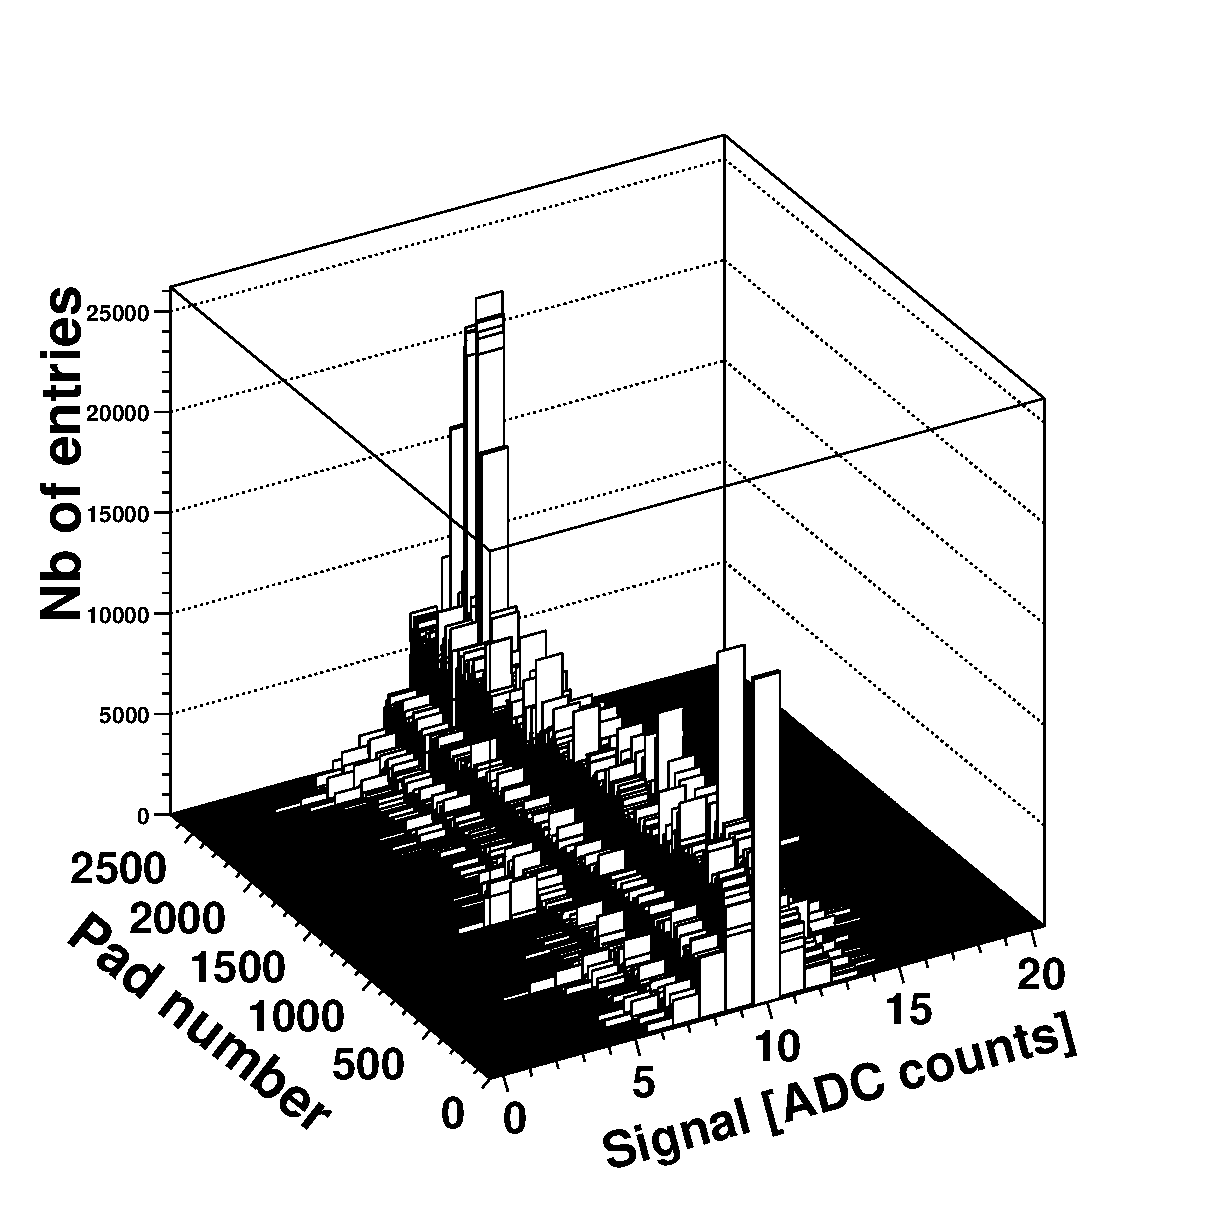
\epsfig{file=plots/baselinenoisedet0run34510ex.eps,width=0.45\textwidth}}
  \caption{\label{baselinenoisedet0run34510ex}2D histogram of the 
detector 0 (SM 0, S0, L0) with the ADC value distributions around 
the baseline (10 ADC counts) for each pad (PEDESTAL run 34510).}
\end{figure}
\subsection{Pedestal algorithm}
During a pedestal run empty events without zero suppression are taken 
with the TRD alone and a random trigger. They are used to determine 
the noise in ADC counts of each pad. The algorithm can be found in the 
{\tt TRDPEDESTALda.cxx} file of the AliRoot TRD directory. It is 
executed on the Local Data Concentrators (LDCs), which are part of the 
dataflow and gives access to sub-events. The TRD has three LDCs 
corresponding to the following blocks of supermodules (SMs):
\begin{itemize}
\item 0-1-2-9-10-11
\item 3-4-5-12-13-14
\item 6-7-8-15-16-17
\end{itemize}   
Three algorithms are therefore executed in parallel during a PEDESTAL 
run for a full installed TRD. After about 100 events, the data-taking 
stops automatically and a 2D histogram is filled for each chamber with 
the ADC amplitude distributions around the baseline for each pad. Such 
a histogram is shown in Fig.\ref{baselinenoisedet0run34510ex} for 
chamber 0 (SM 0 Stack 0 Layer 0).
\begin{figure}[h]
  \centering\mbox{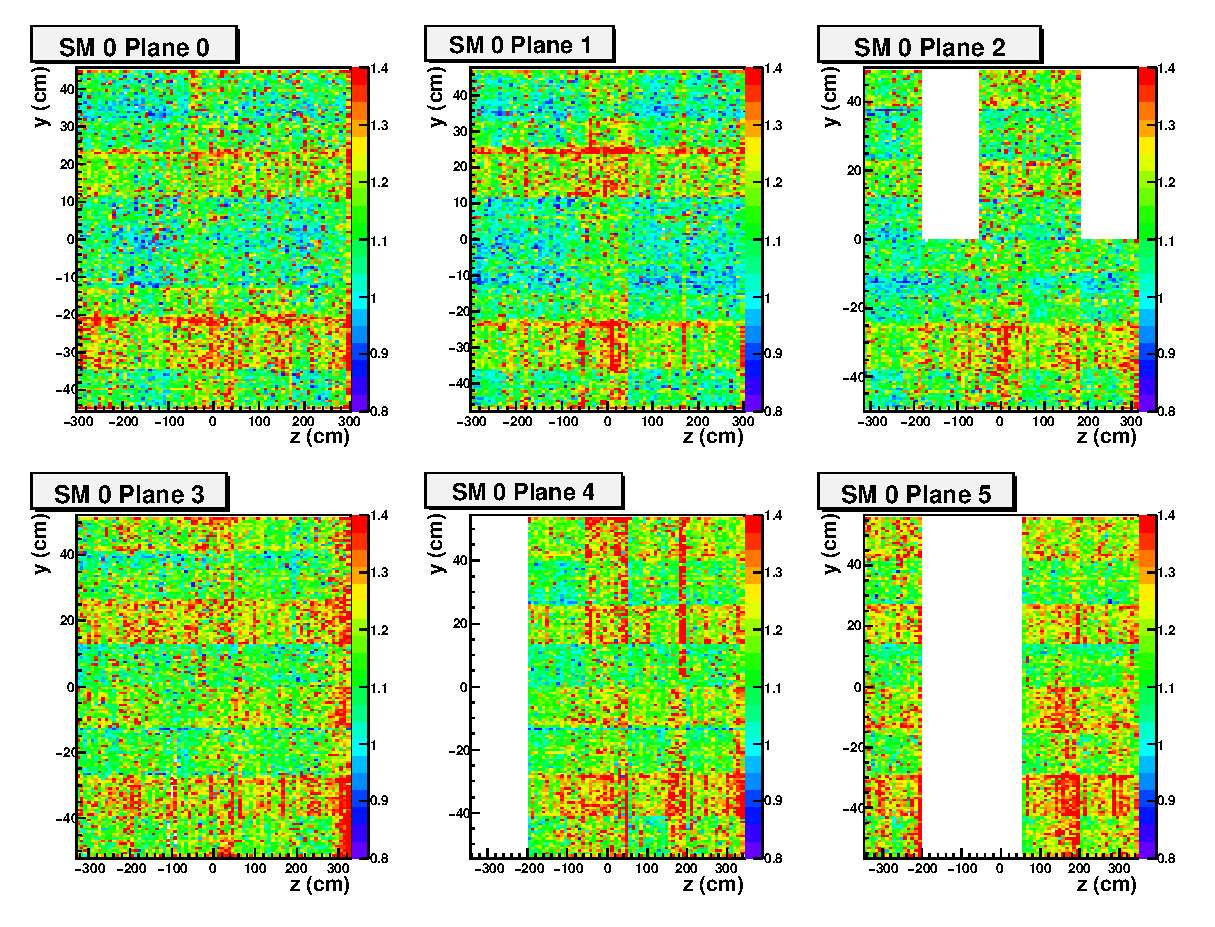
\epsfig{file=plots/run38125sm0nounfold.eps,width=0.88\textwidth,height=0.55\textwidth}}
  \caption{\label{run38125sm0nounfold}Noise in the six planes of 
SM 0 (PEDESTAL run 38125). The five stacks in each layer are in 
the {\it{z}} direction.}
\end{figure}
The chambers should be so configured that the data is without zero 
suppression otherwise an error message appears on the DAQ online 
Logbook. The container class is called {\tt AliTRDCalibPadStatus} 
and allows to further fit the distributions with a Gaussian to 
determine the baseline and noise of each pad. The function is called 
{\tt AliTRDCalibPadStatus::AnalyseHisto()}. In 
Fig.\ref{run38125sm0nounfold} the noise in SM 0 is plotted for the 
PEDESTAL run 38125. It shows stripe patterns of higher noise in the 
$z$-direction (beam direction) correlated to the static pad capacitance 
of the pad plane. The noise distributions has to be first corrected 
for the expected noise variations induced by the pad capacitance 
before a status can be given to each pad. This is not done on the DAQ 
but just before storing the parameters inside the Offline Condition 
Database (OCDB) in the Preprocessor.

\subsection{Drift velocity and timeoffset algorithm}
The drift velocity and timeoffset are calibrated with physics events, 
$pp$ or $PbPb$ collisions. The algorithm is called 
{\tt TRDVDRIFTda.cxx} and can be found in the AliRoot TRD directory. 
It is executed on a dedicated monitoring server, which is not part 
of the dataflow and gives access to full events of the TRD. The 
physics events are used to fill continuously during data-taking an 
average pulse height for each detector. They are stored in a 
{\tt TProfile2D}, which is a member of a { \tt AliTRDCalibraFillHisto} 
object. The {\tt TProfile2D} is written at the end of the run in a 
root file put on the DAQ FXS.\\
\begin{figure}[h]
  \centering\mbox{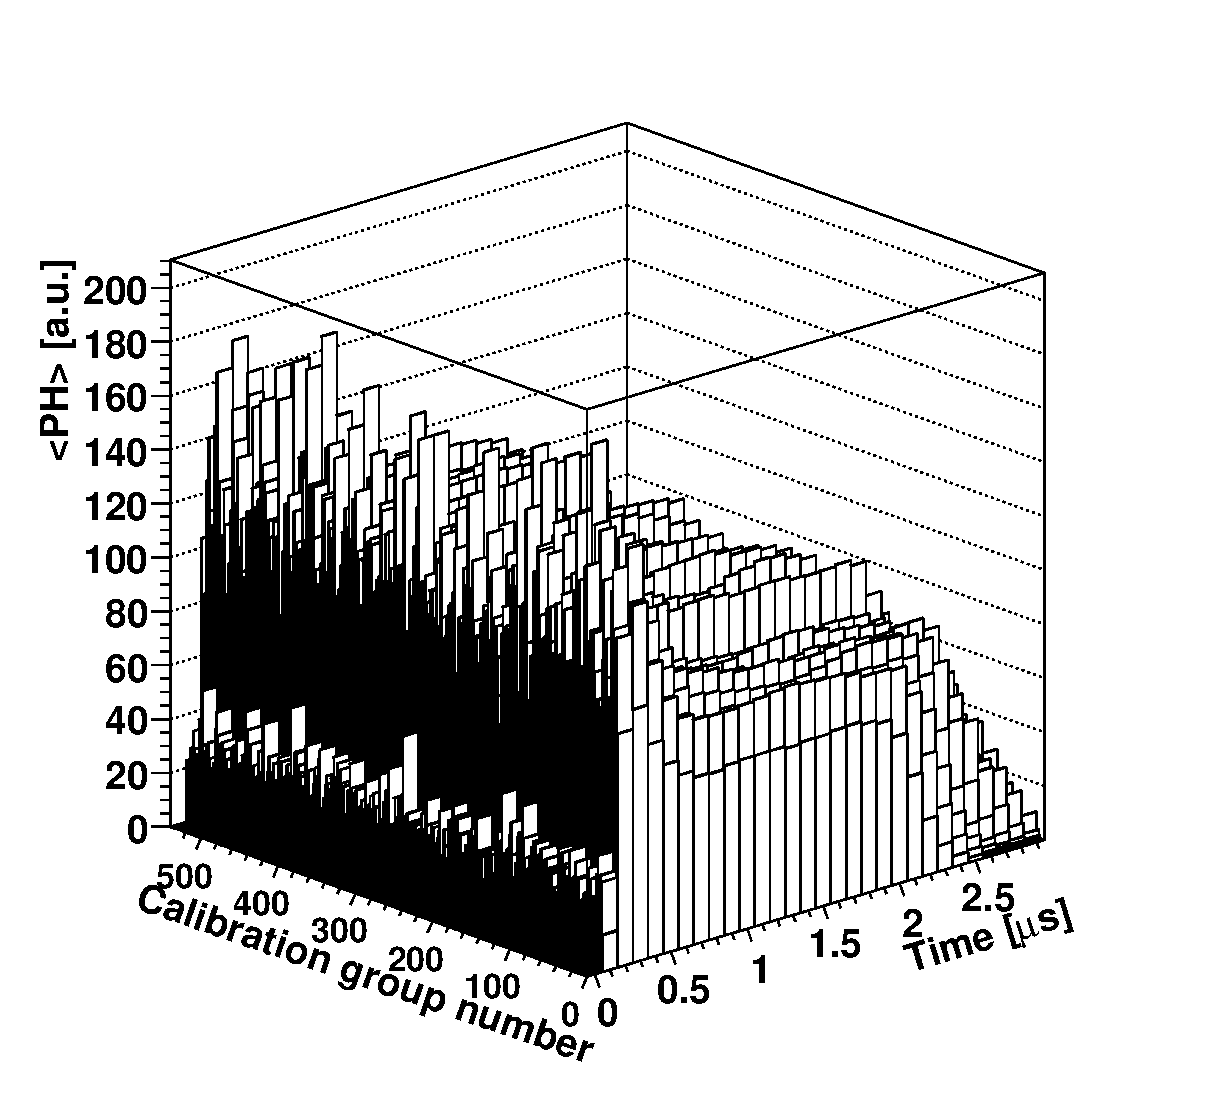
\epsfig{file=plots/referenceph2d.eps,width=0.6\textwidth,,height=0.5\textwidth}}
  \caption{\label{referenceph2d}2D histogram containing the average 
pulse height distributions of each calibration group (here detector), 
produced with decalibrated simulated $pp$ events.}
\end{figure}

Fig.\ref{referenceph2d} shows an output {\tt TProfile2D} obtained 
from simulated decalibrated $pp$ collisions at 14\,TeV. The first 
peak in time corresponds to the amplification region, where the 
contributions of ionization electrons, which come from both sides 
of the anode wire plane, are overlapping. The flat plateau results 
from the electrons in the drift region. The tail is caused by the 
Time Response Function. From this average signal as function of time 
the drift velocity and timeoffset can be extracted by fit procedures. 
This last step is performed in the Preprocessor.\\
Since no tracking is available on DAQ, a simple tracklet finder is 
used. It was optimized for a low charged particle multiplicity 
environment. The algorithm looks for a maximum of the signal 
amplitudes in the chamber after integration over all timebins. The 
average pulse height is then filled for a spot of two pad rows 
($z$ direction) and four pad columns ($r\phi$ direction) around the 
maximum. Further details can be found in the function 
{\tt AliTRDCalibraFillHisto::ProcessEventDAQ}.
%
\section{HLT Calibration}
The High Level Trigger has the big advantage to provide an online 
reconstruction of the events. The idea is then to run the calibration 
procedures in a transparent way, independent whether online or 
offline. The same function 
\\{\tt AliTRDCalibraFillHisto::UpdateHistogramsV1(AliTRDtrackV1 *t)} 
is used to fill the $dE/dx$ distributions (gain), the average pulse 
height (drift velocity and timeoffset) and the Pad Response Function 
for each detector in respectively one {\tt TH2I} and two 
{\tt TProfile2Ds}. The calibration is nevertheless done per chamber, 
whereas by integrating statistics it will be possible to get the gain, 
drift velocity and timeoffset distributions inside the chambers offline. 
Therefore the class {\tt AliTRDCalibraFillHisto} contains a flag 
({\tt fIsHLT}) to avoid extra calculations not needed at the detector 
level.\\
\begin{figure}[hbt]
  \centering\mbox{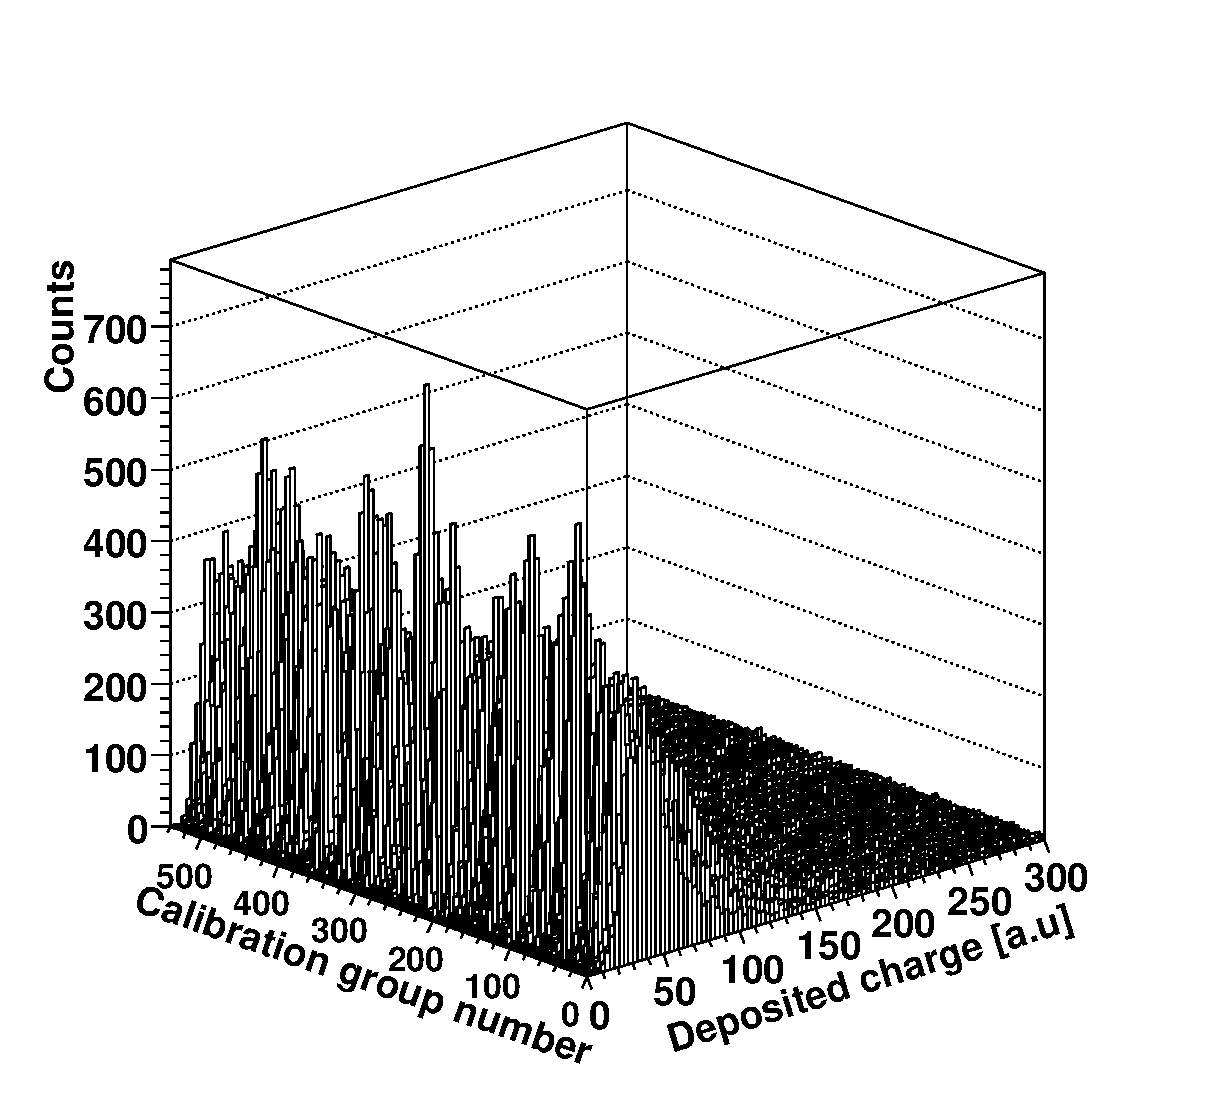
\epsfig{file=plots/referencech2d.eps,width=0.55\textwidth,,height=0.45\textwidth}}
  \caption{\label{referencech2d}A 2D histogram containing the 
$dE$$/$$dx$ distributions of each detector. These were produced 
with decalibrated simulated $pp$ events.}
\end{figure}

Fig.\ref{referencech2d} shows one example of a {\tt TH2I} histogram, 
where the $dE/dx$ distributions of each detector is stored for $pp$ 
collisions at 14\,TeV. No minimal $p_{T}$ cut was applied on the 
TRD tracks. Assuming that the charged particles are uniformy 
distributed over the TRD chambers, the position of the Most Probable 
Value of the $dE/dx$ distribution is used to calibrate the gain.\\ 
At the beginning of each run, a local copy of the OCDB is updated 
on the HLT cluster: the HCDB (HLT Condition Database). The last set 
of calibration objects are used to reconstruct the events. The gain 
correction preformed during the tracking has to be taken into account 
when filling the $dE/dx$ distributions. That is why the calibration 
algorithm has to know which database was used during the 
reconstruction. The TRD HLT code can be found in the {\tt HLT/TRD} 
subdirectory of the AliRoot installation. The calibration is 
implemented as an {\tt AliHLTTRDCalibrationComponent}, whose members 
are an {\tt AliCDBManager} together with the path for the current 
database used, and an {\tt AliTRDCalibraFillHisto} object. The main 
functions are:
\begin{itemize}
\item {\tt AliHLTCalibrationComponent::InitCalibration}, where the 
{\tt TH2I} and {\tt TProfile2Ds} are created.
\item {\tt AliHLTCalibrationComponent::ProcessCalibration}, where 
the function\\ 
{\tt AliTRDCalibraFillHisto::UpdateHistogramsV1(AliTRDtrackV1 *t)} 
is called to fill the histograms.
\item {\tt AliHLTCalibrationComponent::FormOutput}, which returns 
a {\tt TObjArray} with the histograms.
\end{itemize}     
The histograms are shipped at the end of each run to the HLT File 
Exchange Server to be picked up by the SHUTTLE and further processed 
by the Preprocessor, exactly as the data from the calibration on DAQ.
%
\section{Preprocessor}
%
The online systems, like the Detector Control System (DCS), the DAQ 
and the HLT, are protected from outside by a firewall. A special 
framework, called the SHUTTLE, has been developped to retrieve offline 
data in the online systems or store relevant information from the 
online systems in the OCDB. The SHUTTLE has access to the DCS, DAQ 
and HLT FXS. At the end of each run the reference data, outputs of 
the calibration algorithms on DAQ and HLT, are retrieved and further 
processed to determine the calibration constants (gain, drift velocity, 
timeoffset and width of the Pad Response Function). The reference 
data are finally stored in the Grid reference Data Base, whereas the 
results of the fit procedures are stored in the OCDB.\\
The code is contained in the {\tt AliTRDPreprocessor} class. The 
Process function is executed for the run types: PEDESTAL, STANDALONE, 
DAQ and PHYSICS.
\begin{itemize}
\item The PEDESTAL run are dedicated to the calibration of the noise 
on DAQ. Only the output of the DAQ pedestal algorithm is retrieved at 
the SHUTTLE. From the noise and baseline of each pad, a pad status is 
determined. Disconnected pads are recognizable by a small noise. 
Bridged pads have the same noise and baseline. The noise and 
padstatus of the previous pedestal run in the OCDB are taken for half 
chambers, which were not On. Finally the database entries 
{\tt DetNoise}, {\tt PadNoise} and {\tt PadStatus} are populated in 
the OCDB. More informations can be found in the function 
\\{\tt AliTRDPreprocessor::ExtractPedestals}.
\item The STANDALONE runs are used to check the data integrity or the 
correlated noise. The data are taken with the TRD alone and a random 
trigger. Only the DCS data are retrieved.
\item The DAQ run are test runs for the DAQ people. Only the DCS data 
are retrieved.
\item The PHYSICS run are global runs including more than one detector 
and different trigger clusters. They are used for the calibration of 
the gain, driftvelocity and timeoffset, and width of the PRF. Therefore 
the output of the calibration algorihms running on HLT are retrieved. 
If the procedure is not successful the output of the 
driftvelocity$/$timeoffset algorithm on DAQ is also retrieved. The 
reference data, the histograms, are fitted using an 
{\tt ALiTRDCalibraFit} instance:
\begin{itemize}
\item {\tt AliTRDCalibraFit::AnalyseCH(const TH2I *ch)} determines 
the MPVs of the $dE/dx$ distributions and compares them to a reference 
value.
\item {\tt AliTRDCalibraFit::AnalysePH(const TProfile2D *ph)} fits 
the average pulse height and determines the position of the amplification 
region peak and the end of the drift region for each chamber. Knowing 
the length of the drift region one can deduce the drift velocity. The 
amplification peak gives also information on the timeoffset.   
\item {\tt AliTRDCalibraFit::AnalysePRFMarianFit(const TProfile2D *prf)} 
determines the spread of the clusters as function of azimuthal angle of 
the track. The minimum gives the width of the PRF.
\end{itemize}
The results of each fit procedure are stored in a {\tt TObjArray} of 
\\{\tt AliTRDCalibraFit::AliTRDFitInfo} objects, one per chamber, which 
is a member of the {\tt AliTRDCalibraFit} instance. The functions 
{\tt AliTRDCalibratFit::CreateDetObject*} and {\tt ::CreatePadObject*} 
allow to create from the {\tt TObjArray} the final calibration objects, 
that have to be put in the OCDB.
\end{itemize}
Tab.\ref{taskruntype} summarizes the tasks executed by the prepocessor 
for each run type.
\begin{table}[h]
\begin{center}
\begin{tabular} {|c|c|c|c|c|}
\hline run type & DCS data points  & DCS FXS & DAQ FXS & HLT FXS  \\
 & temperatures  & electronic  & calibration DA  & calibration DA   \\
 & voltages, etc $\cdots$  &  configuration & noise/($v_{dE}$$/$$t_{0}$)  
& $g$/($v_{dE}$$/$$t_{0}$)/$\sigma_{PRF}$   \\
\hline DAQ   & yes & yes & no & no \\\hline
\hline PEDESTAL   & no & no & yes (noise) & no \\\hline
\hline STANDALONE & yes & yes & no & no \\\hline
\hline PHYSICS & yes & yes & yes ($v_{dE}$$/$$t_{0}$) & yes \\\hline
\end{tabular} 
\caption{\label{taskruntype} Tasks performed by the TRD preprocessor 
for every run type.} 
\end{center}
\end{table}
The DCS data points are measurements of the currents, voltages, 
temperatures and other variables of the chambers as function of time. 
They are saved in the DCS Archive DB during the run and made available 
at the SHUTTLE by AMANDA.
%
\section{Offline Calibration}
The offline calibration of the gain, driftvelocity$/$timeoffset and 
width of the PRF is meant to improve the first calibration online. 
It follows the following steps:
\begin{itemize}
\item Fill reference data (the $dE/dx$ distributions, the average 
pulse heights $\cdots$) during the reconstruction of the events offline.
\item Store the reference data in root files in AliEn.
\item Merge the reference data of different runs and$/$or calibration groups.
\item Fit the reference data to extract the calibration constants and 
create the calibration objects.
\item Store the calibration objects according to their run validity in 
the OCDB.
\end{itemize}
The calibration procedure is not performed per detector anymore but per 
pad, at least for the first step, the filling of the reference data. 
Depending on the available statics the reference data of different pads 
(calibration groups) can be merged together to determine a mean 
calibration coefficient over these pads.
\subsection{AliTRDCalibraVector container}
The high granularity of the calibration, with a total number of 1181952 
pads, implies that the size of the reference data has to be reduced to 
the strict minimum needed.
\begin{table}[h]
\begin{center}
\begin{tabular} {|c|c|c|}
\hline reference data & Number of  & size  \\
 for & calibration groups  & in MB   \\\hline
 gain & 1181952 & 225 \\\hline
 driftvelocity$/$timeoffset & 1181952 & 271 \\\hline
 PRF  & 131328  & 200 \\\hline
 All together & & 696 \\\hline
\end{tabular} 
\caption{\label{sizeofAliTRDCalibraVector} Size of the 
{\tt AliTRDCalibraVector} object for a given granularity.} 
\end{center}
\end{table}

The {\tt TH2I} and {\tt TProfile2D} objects are not a good option 
anymore. Therefore a container class, {\tt AliTRDCalibraVector}, was 
developped. The {\tt TH2I} corresponds to an array of UShort (2 Bytes) 
for the number of entries in each bin, the {\tt TProfile2D} to an array 
of UShort for the number of entries in each bin and two arrays of Float 
for the sum of the weights and the sum of the squared weights in each 
bin. The mean value and its error are computed per hand in the functions 
{\tt AliTRDCalibraVector::UpdateVector*}, where the object is filled 
with new data. The size of the {\tt AliTRDCalibraVector} object is 
summarized in Tab.\ref{sizeofAliTRDCalibraVector}.\\
%
\subsection{Additional method to calibrate the drift velocity}
In addition an other method is available for the calibration of the 
drift velocity. It is based on the comparison of the slope of the TRD 
tracklet in the azimuthal plane $xy$ with the $\phi$ angle of the 
global track. It can be shown that the slope $dy/dt$ of a TRD tracklet 
depends linearly on its global track parameters, 
$\tan(\phi)+(dz/dx)\tan(\beta_{tilt})$ \cite{THESISR}. The slope 
parameter is the drift velocity in the electric field direction, 
whereas the constant gives the tangent of the Lorentz angle. If the 
TRD tracklet crosses two different pads in the $z$ direction (the 
beam direction), the relation is not true anymore. Therefore such 
tracklets are rejected in the calibration procedure. The reference 
data are a {\tt TObjArray} of one {\tt TH2F} histogram for each 
detector.\\
\begin{figure}[hbt]
  \centering\mbox{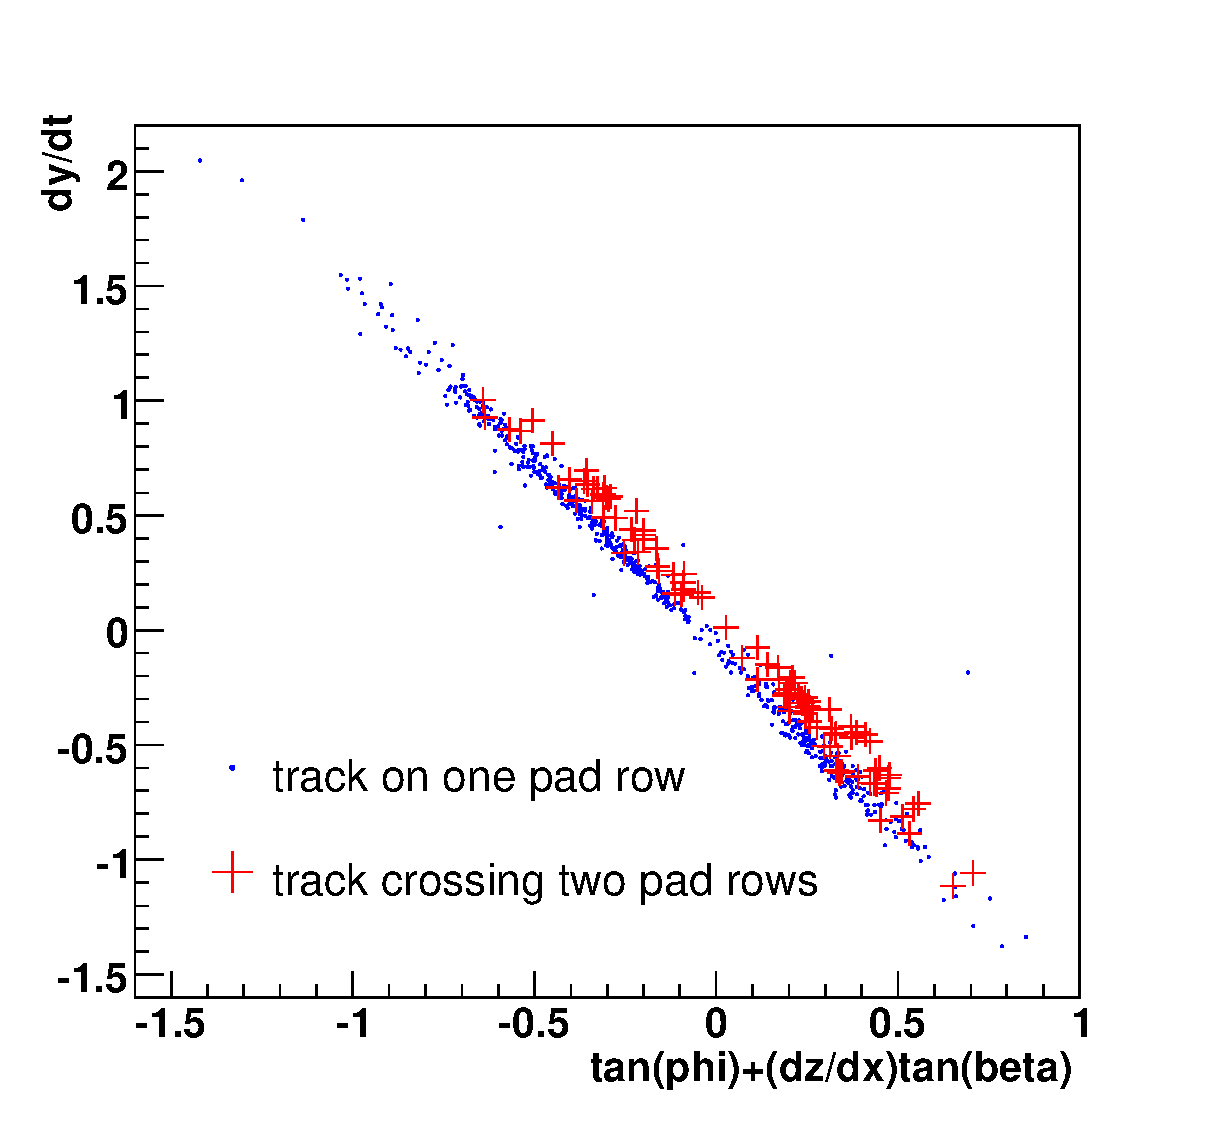
\epsfig{file=plots/crossrow.eps,width=0.5\textwidth,height=0.45\textwidth}}
  \caption{\label{crossrow}The correlation between $dy/dt$ and 
$\tan(\phi)+(dz/dx)\tan(\beta_{tilt})$ for the reconstructed track 
in one chamber. The tracks crossing at least two pad rows are in 
red crosses and those crossing one pad row in blue points.}
\end{figure}

Fig.\ref{crossrow} shows one example of such a histogram. They are 
filled in the function 
\\{\tt AliTRDCalibraFillHisto: :UpdateHistogramsV1(AliTRDtrackV1 *t)}, 
like the reference data for other calibration constants, if the 
flag {\tt fLinearFitterDebugOn} is true.\\
The histograms are stored in the container class, 
\\{\tt AliTRDCalibraVdriftLinearFit}, for which a {\tt Merge} and 
{\tt Add} function have been implemented. In a second step, the 
{\tt AliTRDCalibraVdriftLinearFit} objects can be merged together 
for different runs. In a third step, the {\tt TH2F} histograms are 
fitted in the function \\{\tt AliTRDCalibraVdriftLinearFit::FillPEArray}. 
The result parameters are members of the 
{\tt AliTRDCalibraVdriftLinearFit} object, as well as their error 
coming from the fit procedures. Finally the 
{\tt AliTRDCalibraVdriftLinearFit} object is passed to an 
{\tt AliTRDCalibraFit} instance through the function 
{\tt AliTRDCalibraFit::AnalyseLinearFitters}, in which the Lorentz 
angle is computed from the fit parameters and stored together with 
the drift velocity in a {\tt TObjArray}, member of the 
{\tt AliTRDCalibraFit} instance. As for the other calibration 
constants the functions {\tt AliTRDCalibratFit::CreateDetObject*} 
and {\tt ::CreatePadObject*} allows to create the final calibration 
objects, that have to be put in the OCDB. Since the Lorentz angle 
is not a OCDB entries, it is only used for debugging.
%       
\subsection{The calibration AliAnalysisTask}
The reference data of the calibration are filled in an AliAnalysisTask 
during the reconstruction or after the reconstruction. Since it needs 
some informations only stored in the AliESDfriends, they have to be 
written if one wants to run the calibration. This will be the case 
only for TRD track above a given $p_{T}$ since the size of the events 
is otherwise to big.
%
%%%%%%%%%%%%%%%%%%%%%%%%%%%%%%%%%%%%%%%%%%%%%%%%%%%%%%%%%%%%%%%%%%%%%
\newpage
\setcounter{chapter}{4}
\setcounter{section}{0}    
\Chapter{Alignment}
\thispagestyle{empty}
%
\section{???}
%
%%%%%%%%%%%%%%%%%%%%%%%%%%%%%%%%%%%%%%%%%%%%%%%%%%%%%%%%%%%%%%%%%%%%%
\newpage
\setcounter{chapter}{5}
\setcounter{section}{0}    
\Chapter{Quality Assurance (QA)}
\thispagestyle{empty}
%
\section{???}
%
%%%%%%%%%%%%%%%%%%%%%%%%%%%%%%%%%%%%%%%%%%%%%%%%%%%%%%%%%%%%%%%%%%%%%
\newpage
\setcounter{chapter}{6}
\setcounter{section}{0}    
\Chapter{High Level Trigger (HLT)}
\thispagestyle{empty}
%
\section{???}
%
%%%%%%%%%%%%%%%%%%%%%%%%%%%%%%%%%%%%%%%%%%%%%%%%%%%%%%%%%%%%%%%%%%%%%
\newpage
\setcounter{chapter}{7}
\setcounter{section}{0}    
\Chapter{References}
\thispagestyle{empty}
%
\begin{thebibliography}{99}
%
\bibitem{ALIROOT}  {\it The ALICE Offline Bible}\\
                   http://aliceinfo.cern.ch/export/sites/AlicePortal/Offline/galleries/Download/OfflineDownload/ \\
                   OfflineBible.pdf.
%
\bibitem{CLEMENS}  C.~Adler,
                   {\it Radiation length of the ALICE TRD}
%
\bibitem{DAVID}    D.~Emschermann,
                   {\it Numbering Convention for the ALICE TRD Detector.},
                   http://www.physi.uni-heidelberg.de/\~demscher/alice/numbering/more/TRD\_numbering\_v04.pdf.
%
\bibitem{TRPHOT}   M.~Castellano et al.,
                   Comp. Phys. Comm. {\bf 55}, 431 (1988),
                   Comp. Phys. Comm. {\bf 61}, 395 (1990),
%
\bibitem{DATE}     K.~Schossmaier et al.,
                   {\it The Alice Data Acquisition and Test Environment DATE V5}, 
                   CHEP06.
%
\bibitem{THESISR}  R.~Bailhache, 
                   {\it Calibration of the ALICE Transition Radiation Detector 
                   and a study of $Z^{0}$ and heavy quark production in $pp$ 
                   collisions at the LHC},
                   PhD thesis, University of Darmstadt (Germany), 2009.
%
\end{thebibliography}
%
%%%%%%%%%%%%%%%%%%%%%%%%%%%%%%%%%%%%%%%%%%%%%%%%%%%%%%%%%%%%%%%%%%%%%
%
\end{document}
%%%%%%%%%%%%%%%%%%%%%%%%%%%%%%%%%%%%%%%%%%%%%%%%%%%%%%%%%%%%%%%%%%%%%
